% !TEX root = ../main.tex
\chapter{Quantum Algorithms and Hybrid Variational Architectures}
\label{ch:quantum_algorithms}
{% GRUPPO LOCALE
\renewcommand{\abstractname}{Summary}

\renewenvironment{abstract}{%
  \par\noindent
  {\bfseries\large\abstractname}\par
  \vspace{0.5em}
  \noindent
}{%
  \par\vspace{1em}
}

\begin{abstract}
This chapter explores hybrid quantum--classical machine learning architectures for remote sensing image classification, bridging the Noisy Intermediate-Scale Quantum (NISQ) era with practical applications. We develop a modular \textbf{Quantum Convolutional Neural Network (QCNN)} layer that integrates parameterized quantum circuits into classical convolutional architectures. The QCNN is benchmarked on the EuroSAT satellite imagery dataset and compared against classical CNN baselines. Through systematic ablation studies, we investigate circuit design choices, analyzing their impact on training dynamics, convergence behavior, and classification performance. Results demonstrate that hybrid architectures achieve competitive accuracy (90--95\%) while exhibiting distinctive early-epoch learning characteristics potentially attributable to quantum feature maps. 
\end{abstract}

}


\section{Introduction}
Quantum computing has entered the Noisy Intermediate-Scale Quantum (NISQ) era, with devices
comprising tens to hundreds of noisy qubits~\cite{Preskill2018}. In parallel, deep learning
has become ubiquitous across domains, including satellite-based remote sensing~\cite{Goodfellow2016,Helber2019}.
Hybrid quantum--classical models embed parameterized quantum circuits (PQCs) within neural networks
to potentially augment representation power and learning dynamics~\cite{biamonte2017, cerezo2021}.

Among hybrid models, quantum convolutional neural networks (QCNNs) extend classical convolutions
with quantum kernels for local feature extraction~\cite{Cong2019}. Prior work has explored hybrid
architectures for remote sensing classification~\cite{Sebastianelli2021}, yet the specific role and
design of quantum convolutional layers remain under-explored. This paper develops a QCNN layer,
benchmarks multiple architectures on EuroSAT~\cite{Helber2019}, and compares with a classical CNN
baseline~\cite{LeCun1998} and a published hybrid network~\cite{Sebastianelli2021}. Our contributions are:
(i) a modular QCNN layer compatible with common ML toolchains; (ii) an empirical study of circuit design
choices; and (iii) evidence of distinctive early-epoch learning behavior in QCNNs.

\section{Background}
Hybrid quantum--classical learning integrates short-depth quantum computations\ into a larger classical optimization loop, aiming to exploit quantum resources (superposition, entanglement, and measurement-induced nonlinearities) while remaining compatible with near-term noisy hardware. The conceptual and algorithmic underpinnings are well documented in the monograph by Schuld and Petruccione, which frames quantum models as feature maps and variational learners trained by classical optimizers~\cite{SchuldPetruccione2021}. Complementary surveys emphasize the role of Parameterized Quantum Circuits (PQCs) as flexible hypothesis classes, where the inductive bias, that is, the model’s built-in assumptions about the structure of the target function, emerges from how classical data are encoded into quantum states and from the topology of the entangling gates used. In particular, the choice of encoding scheme and entangling pattern determines the expressivity, trainability, and generalization properties of variational quantum models~\cite{Benedetti2019,cerezo2021}.

\paragraph{Data encoding as a feature map.}
A central design choice is how classical inputs $\mathbf{x}$ are embedded into quantum states. Beyond initialization, \emph{encoding} acts as a feature map $\phi:\mathbf{x}\mapsto \lvert \phi(\mathbf{x})\rangle$ into a high-dimensional Hilbert space, reshaping distances and decision boundaries~\cite{SchuldPetruccione2021,Schuld2019PRA}. Canonical strategies include: (i) \emph{basis encoding}, mapping bits to computational basis states (memory-expensive but simple); (ii) \emph{amplitude encoding}, loading normalized vectors into amplitudes (compact but sensitive to state preparation cost); and (iii) \emph{angle/rotation encoding}, where features modulate rotation angles on single qubits, producing trigonometric feature expansions whose richness grows with depth and entanglement. Interleaving encoders with trainable blocks (\emph{data re-uploading}) probably enhances expressivity by composing nonlinear feature maps with learned unitaries~\cite{PerezSalinas2020,Schuld2020Expressivity}. In many vision-like tasks, locality-aware encodings (e.g., patch-wise rotations) align the quantum hypothesis class with the spatial inductive biases that make classical CNNs effective.

\paragraph{Variational circuits and trainable ans\"atze.}
A PQC defines a unitary  transformation 
\begin{equation*}
U(\boldsymbol{\theta},\mathbf{x})=U_L(\theta_L)\,E(\mathbf{x})\cdots U_1(\theta_1)\,E(\mathbf{x})
\end{equation*}

\noindent that alternates fixed \emph{encoders} $E(\mathbf{x})$ with trainable layers $U_\ell(\theta_\ell)$ (the \emph{ansatz}) and outputs model predictions from expectation values $\langle \hat{O}\rangle$ of suitable observables. Hardware-efficient ans\"atze use native single-qubit rotations and entanglers repeated over shallow depth, while problem-inspired templates inject domain structure via symmetries, locality, or conserved quantities~\cite{Benedetti2019,cerezo2021}. The choice of entangling graph, depth, and encoder placement governs the bias--variance trade-off: too little entanglement limits expressivity; too much depth risks vanishing gradients and noise accumulation.

\paragraph{Forward propagation vs.\ gradient evaluation.}
In classical deep learning, backpropagation reuses intermediate activations via the chain rule across the entire network. In PQC-based models, \emph{forward propagation} consists of executing the circuit and estimating $\langle \hat{O}\rangle$ from a finite number of measurement shots, introducing statistical noise. Crucially, the derivative $\partial \langle \hat{O}\rangle / \partial \theta_k$ is not available by straightforward reverse-mode differentiation through the unitary on hardware; instead, one leverages \emph{parameter-shift} rules that express exact partial derivatives as linear combinations of forward evaluations at shifted parameters (two evaluations per Pauli-generated rotation)~\cite{Mitarai2018,Schuld2019Grad}. This yields unbiased gradients but increases cost roughly proportional to the number of trainable parameters and required shot precision. Simulator-specific \emph{adjoint} methods can reduce cost in silico, but on actual devices the parameter-shift (or closely related) estimators remain the norm. Compared with classical backprop, this gradient acquisition pipeline changes the computational budget and variance profile, motivating shot-frugal schedules and careful layerwise parameterization.

\paragraph{Trainability, noise, and barren plateaus.}
Even with analytic gradients, training can fail when variances vanish (so-called \emph{barren plateaus}), which arise under sufficiently expressive or random ans\"atze, global cost functions, and in the presence of noise~\cite{McClean2018}. Practical recipes emphasize shallow, structured circuits, local cost terms, and encoders that restrict the effective hypothesis class to mitigate concentration-of-measure effects~\cite{SchuldPetruccione2021,cerezo2021}.

\paragraph{Implications for hybrid Q-CNNs.}
These ingredients inform our hybrid quantum convolutional design: (i) patch-wise rotation encoding to respect image locality and to keep state preparation scalable; (ii) shallow entangling blocks arranged in a convolution-like tiling to capture short-range correlations with limited receptive fields; (iii) measurement-defined feature maps serving as quantum ``filters'' whose outputs feed classical layers; and (iv) training via parameter-shift gradients with shot budgeting matched to layer sensitivity. By aligning encoding, ansatz structure, and gradient estimation with the inductive biases of convolutional processing, we obtain architectures that are both hardware-aware and well-posed for the benchmarks presented in the following sections (see Fig.~\ref{fig:hybrid_overview}). 
\begin{figure}[htbp]
    \centering
    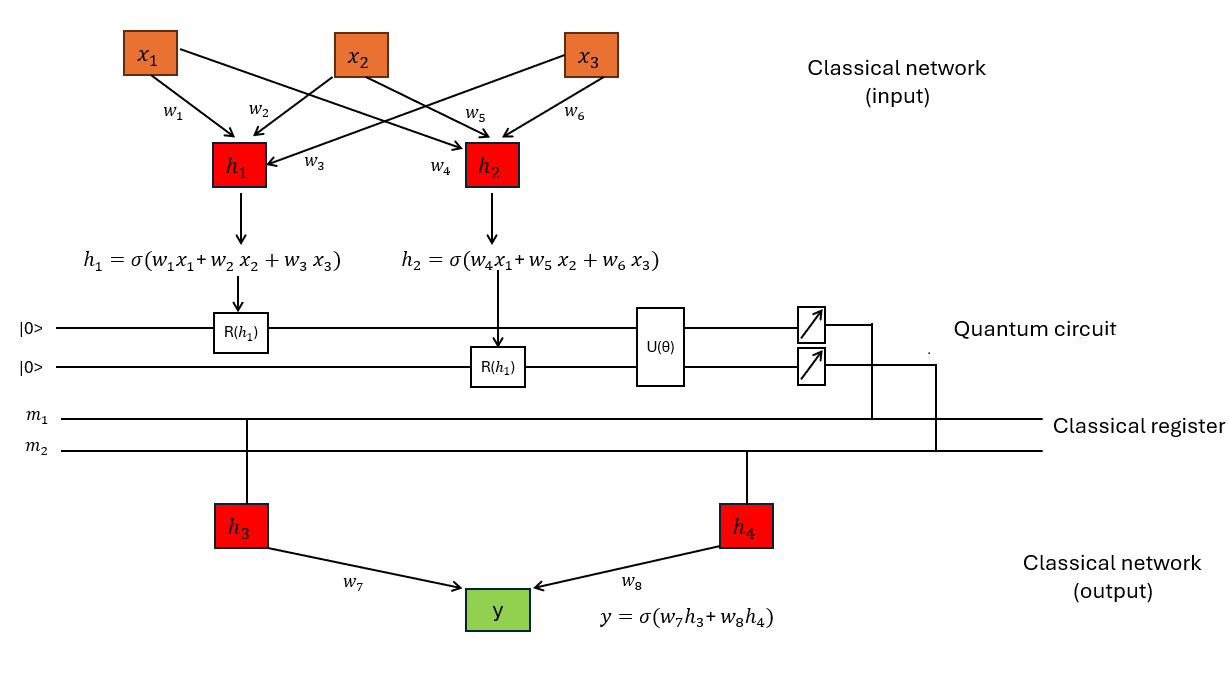
\includegraphics[width=0.9\textwidth]{chapters/qa_figures/intro_ql.png}
    \caption{Schematic representation of a hybrid quantum--classical neural network. 
    Classical features $x_1,x_2,x_3$ are mapped to hidden activations $h_1,h_2$, 
    encoded into qubit rotations $R(h_1)$ and $R(h_2)$, and processed by a variational 
    quantum circuit $U(\boldsymbol{\theta})$. Measured outputs $m_1,m_2$ are passed to a 
    classical readout layer producing the final output $y$. 
    Adapted from~\cite{Filippi2025Thesis}.}
    \label{fig:hybrid_overview}
\end{figure}


\subsection{Classical CNNs}\label{sec:classical-cnns}
Convolutional neural networks (CNNs) exploit locality and weight sharing to extract
translation–equivariant features from images~\cite{Goodfellow2016,LeCun1998}.
Let $\mathbf{X}\!\in\!\mathbb{R}^{H\times W\times C_{\mathrm{in}}}$ be an input and
$\mathbf{K}\!\in\!\mathbb{R}^{k_h\times k_w\times C_{\mathrm{in}}\times C_{\mathrm{out}}}$ a bank of filters.
A 2D convolution produces feature maps $\mathbf{Y}\in\mathbb{R}^{H'\times W'\times C_{\mathrm{out}}}$
via
\begin{equation}
Y_{i,j,c} \;=\; b_c \;+\!
\sum_{u=0}^{k_h-1}\sum_{v=0}^{k_w-1}\sum_{d=0}^{C_{\mathrm{in}}-1}
K_{u,v,d,c}\; X_{i+u,\,j+v,\,d},
\label{eq:conv2d}
\end{equation}
optionally followed by a pointwise nonlinearity $\sigma$, e.g.\ $\mathrm{ReLU}(z)=\max(0,z)$.
Spatial downsampling (pooling) aggregates over local neighborhoods $\Omega$,
\begin{equation}
P_{i,j,c} \;=\; \max_{(u,v)\in\Omega} Y_{s\,i+u,\,s\,j+v,\,c},
\end{equation}
controlling receptive fields while reducing resolution and computation.

For a classifier with logits $\mathbf{z}_n$ and one–hot targets $\mathbf{t}_n$, the cross–entropy objective is
\begin{equation}
\mathcal{L} \;=\; -\frac{1}{N}\sum_{n=1}^{N}\sum_{c=1}^{C}
t_{n,c}\,\log\!\left(\frac{e^{z_{n,c}}}{\sum_{c'} e^{z_{n,c'}}}\right).
\end{equation}
Parameters are updated by (stochastic) gradient descent using backpropagation,
which applies the chain rule layer–wise and reuses intermediate activations efficiently~\cite{Goodfellow2016}.
In our comparisons we adopt a compact LeNet–5–style baseline as a strong, well–understood reference~\cite{LeCun1998}.



\subsection{Quantum Machine Learning and QCNNs}\label{sec:qml-qcnn}
Quantum Machine Learning (QML) models embed classical data into quantum states and process them
with \emph{parameterized quantum circuits} (PQCs) trained by a classical optimizer~\cite{SchuldPetruccione2021,cerezo2021}.
A typical pipeline prepares an encoded state $U_{\phi}(\mathbf{x})\ket{0}$, applies a trainable ansatz $U(\boldsymbol{\theta})$,
and returns an expectation value of an observable $\hat{O}$:
\begin{equation}
\hat{y}(\mathbf{x};\boldsymbol{\theta}) \;=\;
\bra{0}\,U_{\phi}^{\dagger}(\mathbf{x})\,U^{\dagger}(\boldsymbol{\theta})\,
\hat{O}\,U(\boldsymbol{\theta})\,U_{\phi}(\mathbf{x})\,\ket{0}.
\label{eq:q-model}
\end{equation}
Encoding choices include \emph{basis} encoding, \emph{amplitude} encoding,
and \emph{angle} (rotation) encoding, possibly in a \emph{data re–uploading}
pattern that interleaves encoders and trainable layers to enrich expressivity~\cite{SchuldPetruccione2021,PerezSalinas2020,Schuld2020Expressivity}.
For generators with $\pm 1$ eigenvalues, gradients admit the parameter–shift rule~\cite{Mitarai2018,Schuld2019PRA}:
\begin{equation}
\frac{\partial}{\partial \theta_k}\,\hat{y}(\mathbf{x};\boldsymbol{\theta})
\;=\; \tfrac{1}{2}\!\left[
\hat{y}\!\left(\mathbf{x};\boldsymbol{\theta}_{k}^{+}\right)
-\hat{y}\!\left(\mathbf{x};\boldsymbol{\theta}_{k}^{-}\right)\right],
\qquad
\boldsymbol{\theta}_{k}^{\pm}:\ \theta_k \mapsto \theta_k \pm \tfrac{\pi}{2}.
\label{eq:psr}
\end{equation}

\paragraph{QCNNs.}
Quantum convolutional neural networks (QCNNs) implement hierarchical, locality–aware processing
with shallow, repeating blocks that mirror convolution and pooling~\cite{Cong2019}.
Let $\rho^{(\ell)}$ denote the layer–$\ell$ state on a 1D register.\footnote{For 2D images we
tile registers/patches analogously.} A QCNN layer applies a local unitary $W^{(\ell)}$
over neighboring qubits and discards (traces out) pooled subsystems, yielding
\begin{equation}
\rho^{(\ell+1)} \;=\; \mathrm{Tr}_{\mathrm{pool}}
\!\left[\,W^{(\ell)}\,\rho^{(\ell)}\,W^{(\ell)\dagger}\right],
\label{eq:qcnn-pooling}
\end{equation}
which reduces degrees of freedom while propagating entanglement to coarser scales (MERA–like hierarchy~\cite{Cong2019,Vidal2007MERA}).
Measurements of local observables at each scale provide quantum ``feature maps'' that feed subsequent
quantum or classical processing. The choice of encoding $U_{\phi}$ on patches, entangling topology in $W^{(\ell)}$,
and measurement set $\{\hat{O}\}$ governs the inductive bias and the shot/gradient budget.
Feature–map perspectives (e.g.\ kernel embeddings) clarify how certain encoders may induce
advantageous geometries for classification~\cite{Havlicek2019,Schuld2019PRA}.

\paragraph{Forward vs.\ backward.}
Unlike classical backpropagation, which shares intermediates across parameters, hardware gradient evaluation relies on additional circuit executions (Eq.~\ref{eq:psr}) and finite–shot estimation,
impacting sample efficiency and training dynamics~\cite{Schuld2019PRA,SchuldPetruccione2021}.
Consequently, QCNN design favors shallow, locality–preserving ans\"atze with encoders aligned to image patches,
which we operationalize in the Methods and Experiments sections.

\section{Methods}

Our quantum convolutional layer maps small image patches to expectation values via a PQC composed of:
(i) angle (rotation) encoding of pixel intensities; (ii) a hardware-efficient entangling ansatz~\cite{Kandala2017};
and (iii) Pauli measurements whose outcomes form the convolved feature map. In our implementation we employ
Qiskit's \texttt{ZFeatureMap} and custom two-qubit entanglers~\cite{Qiskit2019}.
Device models and timings used throughout are taken from Qiskit \emph{BackendV2}/\emph{Target}~\cite{QiskitBackendV2Docs,QiskitTargetDocs}.


\subsection{Quantum Convolutional Layer}
We realize a quantum convolution as a local, patch-wise mapping from pixels to expectation values computed by a parameterized quantum circuit (PQC). For an image $X\!\in\![0,1]^{H\times W}$ and a sliding window of size $k\times k$ and stride $s$, each vectorized patch $\mathbf{p}\in\mathbb{R}^{d}$ with $d=k^2$ is transformed into $C$ quantum ``channels''
\begin{equation}
\phi_{\boldsymbol{\theta}}(\mathbf{p}) \;=\; \big(\langle M_1\rangle_{\mathbf{p},\boldsymbol{\theta}},\dots,\langle M_C\rangle_{\mathbf{p},\boldsymbol{\theta}}\big),\qquad
\langle M_c\rangle_{\mathbf{p},\boldsymbol{\theta}} \;=\; \bra{0}U^\dagger(\mathbf{p},\boldsymbol{\theta})\,M_c\,U(\mathbf{p},\boldsymbol{\theta})\ket{0},
\label{eq:qconv-core}
\end{equation}
where $M_c$ are Pauli observables and $U(\mathbf{p},\boldsymbol{\theta})=W(\boldsymbol{\theta})\,S(\mathbf{p})$ splits data encoding $S$ from the trainable ansatz $W$ \cite{Benedetti2019,cerezo2021}.
As illustrated in Fig.~\ref{fig:qconv_schematic}, the proposed QConv layer
follows the structure of a variational quantum circuit, where each image patch is encoded into a quantum state via a rotation-based feature map,
processed by a trainable variational ansatz, and measured to obtain expectation
values that act as quantum-derived features for the classical CNN. Hence, 
$W(\boldsymbol{\theta})$ is a trainable block that we realize as a product of \emph{G-blocks}
\begin{equation*}
W(\boldsymbol{\theta}) \;=\; \overleftarrow{\prod_{\ell=1}^{L}} \;\Bigg(\; \prod_{i \in \mathcal{G}_{\ell}} G_{i}^{(\ell)} \Bigg),
\end{equation*}
with the left arrow indicating that blocks at larger $\ell$ are applied later (i.e., rightmost acts first).

\begin{figure}[htbp]
    \centering
    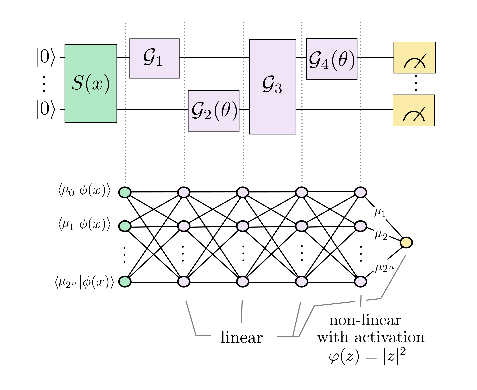
\includegraphics[width=0.85\linewidth]{chapters/qa_figures/Fig5_16_SchuldPetruccione2021.eps}
    \caption{Schematic representation of a variational quantum circuit interpreted 
    as a neural network, adapted from Fig.~5.16 in \cite{SchuldPetruccione2021}. 
    The diagram highlights the correspondence between classical input patches,
    quantum feature encoding, trainable unitary layers, and measurement outputs,
    analogous to the proposed quantum convolutional layer.}
    \label{fig:qconv_schematic}
\end{figure}

The general workflow follows the principle outlined in~\cite{SchuldPetruccione2021}, 
where each parametrized quantum circuit acts as a non-linear feature extractor,
and its measurement outcomes provide a compact representation for classical
post-processing.


In the baseline, we adopt rotation (angle) encoding,
\begin{equation}
S(\mathbf{p}) \;=\; \bigotimes_{i=1}^{d} R_y\!\big(\alpha\,\tilde p_i\big), \qquad \tilde p_i = \frac{p_i-\mu}{\sigma},
\label{eq:angle-enc}
\end{equation}
with a global scale $\alpha$ to adapt the dynamic range. This is hardware-friendly and produces a rich trigonometric feature expansion whose frequency support can be amplified by depth and data re-uploading. Two possibly useful alternatives to explore are: (i) \emph{amplitude encoding}, $|\psi(\mathbf{p})\rangle = \sum_{i} (p_i/\|\mathbf{p}\|_2)\,|i\rangle$, which is qubit-efficient but requires nontrivial state preparation; and (ii) \emph{kernel/phase feature maps} (e.g., IQP-style) that implement problem-inspired kernels via commuting entanglers and data-dependent phases \cite{Havlicek2019, Schuld2020Expressivity}. 
The $U(\mathbf{p},\boldsymbol{\theta})$ decomposition is, as a matter of fact, a way to increase expressivity without extra qubits, through \emph{data re-uploading}:
\begin{equation}
U(\mathbf{p},\boldsymbol{\theta}) \;=\; \prod_{\ell=1}^{L}\Big[\, W_\ell(\boldsymbol{\theta}_\ell)\,S(\mathbf{p}) \,\Big],
\label{eq:reupload}
\end{equation}
which composes encoders with learnable layers, enlarging the accessible Fourier spectrum \cite{PerezSalinas2020, Schuld2020Expressivity}.

The trainable block is a hardware-efficient ansatz,
\begin{equation}
W(\boldsymbol{\theta}) \;=\; \prod_{\ell=1}^{D}\Big[\;\mathcal{E}_\ell\,\bigotimes_{i=1}^{d} R_z(\theta_{\ell i}^{(z)})\,R_x(\theta_{\ell i}^{(x)})\;\Big],
\label{eq:hea}
\end{equation}
where $\mathcal{E}_\ell$ applies short-range entanglers (e.g., linear/ring CNOTs). Entanglement couples pixels within a patch, enabling non-separable features akin to classical cross-channel mixing, but excessive expressibility can harm trainability (Sec.~\ref{sec:train-opt}) \cite{Cong2019,Holmes2022PRXQ,Marrero2021PRXQ}. The shot-based estimator for each channel uses $S$ repetitions:
\begin{equation}
\widehat{\langle M_c\rangle} \;=\; \frac{1}{S}\sum_{s=1}^{S} m_{c,s},\quad m_{c,s}\in\{-1,+1\},\qquad
\mathrm{Var}\big[\widehat{\langle M_c\rangle}\big] \;=\; \frac{1-\langle M_c\rangle^2}{S}.
\label{eq:shotvar}
\end{equation}
Placing the vectors $\phi_{\boldsymbol{\theta}}(\mathbf{p})$ on the patch grid yields a tensor of size $H'\times W'\times C$ (stride- and padding-dependent) that serves as the quantum analogue of a convolutional activation and feeds subsequent (classical or quantum) layers \cite{LeCun1998,Cong2019}.

\textbf{Design notes and upgrades.} (a) Mix $R_y$ and $R_z$ encodings per wire to diversify frequency content; (b) use small, overlapping patches to share context; (c) add a lightweight pooling step by measuring and discarding selected qubits to form multiscale features, inspired by QCNN/MERA \cite{Cong2019,Pesah2021PRX}. 
%We will compare angle-only, angle+phase, and re-uploading variants in Sec.~3.2.


\subsection{QCNN Architectures}
We explore where to insert the quantum layer (early vs late), the number of channels (repetitions per patch),
and circuit depth. These factors control expressivity and generalization~\cite{Benedetti2019,cerezo2021}.
Dropout and batch normalization are used in the classical stack~\cite{Goodfellow2016}.

\paragraph{Inserting quantum layers and shaping their capacity.}
Denote by $\mathrm{QConv}(k,C,D,L)$ a quantum layer using $k{\times}k$ patches, $C$ channels, depth $D$ and $L$ re-uploading cycles (Eqs.~\ref{eq:reupload}–\ref{eq:hea}) (see Fig.~\ref{fig:qconv}). 
\begin{figure}[htbp]
    \centering
    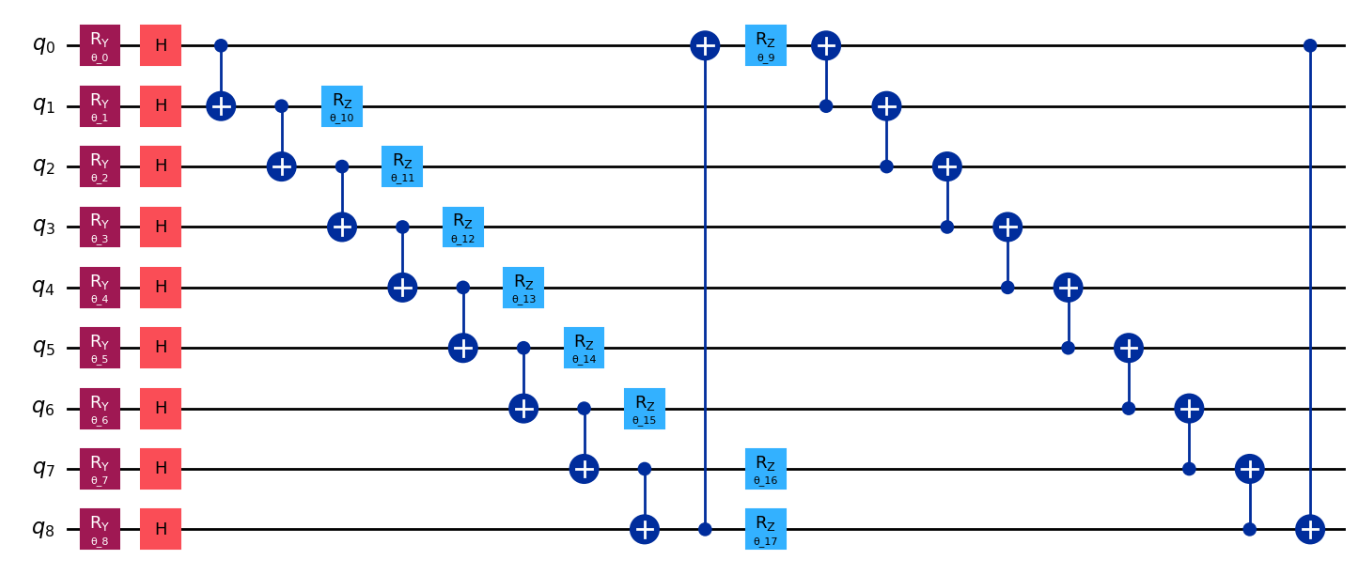
\includegraphics[width=0.95\textwidth]{chapters/qa_figures/conv_circuit.png}
    \caption{TwoLocal ansatz used in the quantum convolutional layer, consisting of 
    nine qubits and alternating $R_Y$/$R_Z$ rotations followed by chains of CNOT 
    entangling gates. The circuit depth $L$ corresponds to the number of alternating 
    layers applied. 
    Adapted from~\cite{Filippi2025Thesis}.}
    \label{fig:qconv}
\end{figure}


We extract local patches of side-length $k$ (i.e., $k\times k$), with $c_{\text{in}}$ input channels, and
flatten them into $d$-dimensional feature vectors, where
$d \;=\; k^2\,c_{\text{in}}$ or the post-projection dimension, if a linear reduction is applied.

Each $d$-dimensional vector is encoded into a $D$-qubit register via a data-encoding unitary
$U_{\text{enc}}:\mathbb{R}^{d}\to \mathrm{SU}(2)^{\otimes D}$ (see Fig.~\ref{fig:qcnn_ansatz}).
\begin{figure}[htbp]
    \centering
    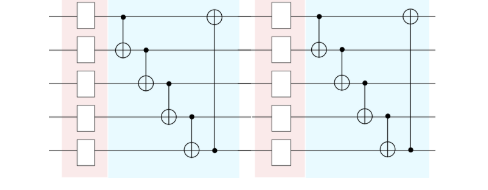
\includegraphics[width=0.8\textwidth]{chapters/qa_figures/basic_entangled.png}
    \caption{Variational quantum circuit based on rotational encoding and entangling 
    CNOT topology, analogous to a fully connected layer in classical neural networks. 
    Each qubit undergoes a sequence of parameterized rotations followed by 
    entanglement with neighboring qubits. 
    Adapted from~\cite{Filippi2025Thesis}.}
    \label{fig:qcnn_ansatz}
\end{figure}


The variational block then applies
$L$ layers of trainable unitaries $U(\boldsymbol{\theta})$, followed by Pauli measurements to produce
$C_q$ quantum feature maps per spatial location. The number of shots per measured channel is $S$.

Two insertion patterns are particularly meaningful: \begin{itemize}
\item \emph{early-fusion} ($\mathrm{QConv}\!\to\!\mathrm{Conv}\!\to\!\cdots$), which exposes the classical trunk to quantum-enriched local features, and 
\item \emph{late-fusion} ($\mathrm{Conv}\!\to\!\cdots\!\to\!\mathrm{QConv}\!\to\!\text{head}$), which turns higher-level classical features into compact quantum embeddings and measurements. 
\end{itemize}
Let the per-patch parameter count be $T\!=\!2D d$ for the rotation layers in Eq.~\ref{eq:hea} (ignoring entangler choices) and total parameters $\mathcal{O}(C\,T)$; capacity scales linearly in $C$ and $D$.

\paragraph{Pooling and hierarchy.}
As previously stated, QCNNs provide a principled way to compress representations by tracing out measured qubits. If $\rho^{(\ell)}$ is the state at layer $\ell$ and $W^{(\ell)}$ acts on local neighborhoods, the next scale is
\begin{equation}
\rho^{(\ell+1)} \;=\; \mathrm{Tr}_{\mathrm{pool}}\!\left[\,W^{(\ell)}\;\rho^{(\ell)}\;W^{(\ell)\dagger}\right],
\label{eq:qcnn-pool}
\end{equation}
reducing width while propagating entanglement to coarser receptive fields (a MERA-like hierarchy) \cite{Cong2019}. Practically, we implement a ``quantum stride'' by computing a subset of observables per patch and discarding the rest, aligning the spatial downsampling with the entangling light-cone.

\paragraph{Entanglement range vs.\ generalization.}
Local entanglers (nearest-neighbor CNOTs) match the short-range statistics of natural scenes and help avoid overly expressive, 2-design-like behavior that correlates with vanishing gradients \cite{Holmes2022PRXQ}. QCNN-style locality and logarithmic depth guarantee that gradients need not vanish exponentially with system size, improving trainability relative to global ansätze \cite{Pesah2021PRX}. Empirically, moderate $D$ (1–3) and small $k$ (2–4) give the best accuracy-to-variance trade-off on EuroSAT while preserving hardware viability.


\paragraph{Alternate ans\"atze and hybrids.}
Three practical enhancements: 
\begin{itemize}
\item{(i)} \emph{Data re-uploading stacks} (Eq.~\ref{eq:reupload}) to boost spectral richness without extra qubits \cite{PerezSalinas2020,Schuld2020Expressivity}; \item{(ii)} \emph{kernel-style encoders} on patches (commuting phase layers) feeding a shallow $W(\theta)$ for stability \cite{Havlicek2019}; 
\item{(iii)} \emph{serial hybrids}
$\mathrm{Conv}\!\to\!\mathrm{QConv}\!\to\!\mathrm{Conv}$, where the first classical block denoises, the quantum layer mixes nonclassically, and the last classical block refines decision boundaries \cite{LeCun1998}. 
\end{itemize}
When resources allow, a small second $\mathrm{QConv}$ after classical pooling can capture larger-scale correlations without a large qubit count by using bigger strides.

In contrast to the data re-uploading strategy~\cite{PerezSalinas2020}, 
our quantum convolutional layer employs a single data-encoding stage followed by $L$ trainable variational blocks, 
without re-injecting classical inputs at each layer.
This design mirrors the locality and weight-sharing principles of classical convolution kernels,
while reducing the number of parameters and mitigating barren plateau effects~\cite{cerezo2021}.


\paragraph{Complexity.}
For each patch and channel, we need $S$ shots per observable; a full forward pass costs $\mathcal{O}(N_{\mathrm{patch}}\,C\,L\,D\,S)$ circuit evaluations. Late-fusion reduces $N_{\mathrm{patch}}$ because it acts on feature maps of smaller spatial size; early-fusion may provide a stronger signal to the classical trunk. In our experiments, we report both patterns and ablations over $C, D, L$ to measure accuracy vs.\ variance vs.\ time.
\paragraph{Ablation studies.}
To assess the relative contribution of circuit width, depth, and output dimensionality,
we performed a set of ablation studies varying the number of qubits ($D$), 
variational layers ($L$), and quantum channels ($C$) while keeping all other settings fixed. 
Each configuration was trained over ten runs to evaluate accuracy, variance, and runtime. 
We also compared early- and late-fusion schemes, isolating the effect of the 
insertion point of the quantum layer on overall model performance and computational cost.


\subsection{QCNN model}



\subsection{Dataset and Preprocessing}
\label{sec:dataset-and-preprocessing}
We use EuroSAT (Sentinel-2) with $64{\times}64$ tiles and evaluate a binary subset to isolate the effect of quantum feature extraction \cite{Helber2019,Sebastianelli2021}. We keep the classical and hybrid pipelines as comparable as possible.
In this work, we limited the analysis to a binary subset of the EuroSAT dataset, 
comprising two of the ten available classes from the original 27{,}000-image collection, 
as a trade-off between architectural simplicity and computational feasibility.


\paragraph{Band selection and scaling.}
For RGB experiments we extract the three visible bands; for multispectral variants we pick physically motivated composites (e.g., adding NIR) that accentuate vegetation/soil contrasts. All images are resized to $H{\times}W$ divisible by the stride $s$ and normalized per image:
\begin{equation}
\tilde x \;=\; \frac{x-\mu}{\sigma},\qquad \mu=\frac{1}{HW}\textstyle\sum_{i,j}\!x_{ij},\quad
\sigma^{2}=\frac{1}{HW}\sum_{i,j}(x_{ij}-\mu)^2.
\end{equation}
Rotation encodings use $\theta=\alpha\,\tilde x$ (Eq.~\ref{eq:angle-enc}), while phase maps use $\varphi=\beta\,\tilde x$ to keep phases within $[-\pi,\pi]$.

\paragraph{Patch extraction and channels.}
We extract vectorized patches $\mathbf{p}\in\mathbb{R}^{k^2}$ with kernel $k\!\in\!\{2,3,4\}$ and stride $s\!\in\!\{1,2\}$. Overlap (small $s$) increases context at the cost of more circuits. Multi-channel outputs can be realized by (a) different observables $M_c$ on the same wires, or (b) channel-specific ansätze $W_c(\theta_c)$ with shared $S(\mathbf{p})$. The latter increases capacity but also shots and parameter budgets.

\paragraph{Augmentation and splits.}
We apply light augmentations (horizontal/vertical flips, $\pm 10^\circ$ rotations) equally to classical and hybrid models. The dataset is stratified into 80\% train and 20\% validation, balanced per class. Batches mix patches from multiple images to reduce inter-sample correlations
and approximate $\mathbf{i}$ndependent and $\mathbf{i}$dentically $\mathbf{d}$istributed (i.i.d.) sampling, ensuring unbiased gradient estimates for the classical head.
\cite{Goodfellow2016}.

\paragraph{Why encoding design matters here.}
Angle encodings are robust and cheap; re-uploading can significantly improve fit in low-depth settings by enriching the frequency content \cite{PerezSalinas2020,Schuld2020Expressivity}. Kernel-style feature maps (e.g., data-dependent ZZ-phases on neighboring wires) induce inner-product geometries beneficial for some land-use separations \cite{Havlicek2019}. We used angle-only encoding and leave to future work to compare: (i) angle-only; (ii) angle+phase; (iii) re-uploaded angle. For completeness, it should also be benchmarked a small amplitude-encoding variant on downsampled patches to assess the trade-off between state-prep cost and qubit efficiency.

\paragraph{Outputs for downstream heads.}
The quantum feature tensor $F\in\mathbb{R}^{H'\times W'\times C}$ feeds either a shallow classical CNN head or a linear classifier. We matched heads across baselines so that performance differences reflect the quantum layer rather than a stronger classical readout. This way, we kept the readout capacity normalized so that any gain is due to the quantum convolution, not a stronger classifier.


\subsection{Training and Optimization}\label{sec:train-opt}
Our optimization protocol is staged. First, we conduct architecture search and hyperparameter tuning entirely on \emph{simulators} within the Qiskit ecosystem, selecting a single best candidate per setting. Second, we aim to conduct a limited set of \emph{hardware validations} on an IQM superconducting device (54 qubits) accessed via Qiskit, to assess its robustness under realistic noise and topology constraints (on-going activity).

\paragraph{Objective and gradient evaluation.}
Let $f_{\boldsymbol{\theta}}(X)$ denote the logit produced after pooling the quantum feature tensor and a linear head. For binary tasks we minimize cross-entropy
\begin{equation}
\mathcal{L}(\boldsymbol{\theta})
= -\frac{1}{N}\sum_{n=1}^{N}\!\big[y_n\log \sigma(f_{\boldsymbol{\theta}}(X_n)) + (1-y_n)\log \!\big(1-\sigma(f_{\boldsymbol{\theta}}(X_n))\big)\big],
\end{equation}
and compute PQC gradients with the \emph{parameter-shift} rule \cite{Schuld2019PRA,Mitarai2018}: for gates generated by Pauli operators,
\begin{equation}
\frac{\partial}{\partial \theta_j}\,\langle M\rangle_{\boldsymbol{\theta}}
= \tfrac{1}{2}\Big(\,\langle M\rangle_{\theta_j+\tfrac{\pi}{2}} - \langle M\rangle_{\theta_j-\tfrac{\pi}{2}}\,\Big),
\label{eq:psr-34}
\end{equation}
so each partial derivative requires two additional forward evaluations. On Qiskit, we use the \emph{Estimator} primitive to obtain expectation values consistently across simulators and hardware backends \cite{QiskitEstimatorDocs,Qiskit2019}. With $s$ shots per expectation, the variance of the estimator scales as
\begin{equation}
\mathrm{Var}\!\left[\widehat{\langle M\rangle}\right] \;=\; \frac{1-\langle M\rangle^2}{s},
\qquad
\mathrm{SE}\!\left[\widehat{\langle M\rangle}\right] \;=\; \mathcal{O}(S^{-1/2}),
\label{eq:shot-var-34}
\end{equation}
Hence, we schedule $S$ to increase during training (low $S$ for exploration, high $S$ for convergence) to lower Standard Error (SE).

\paragraph{Simulator-first search (Qiskit).}
For relatively rapid prototyping, we rely on Qiskit Aer backends. Where relevant, we use (i) exact statevector simulation for sanity checks (no sampling noise), (ii) shot-based simulation to match the training signal of hardware, and (iii) device-aware transpilation (layout and coupling map) to estimate depth and two-qubit counts faithfully. For IQM-targeted experiments, we employ the IQM Qiskit adapter to simulate circuits with IQM-specific noise models (when available) and topology, so that the selected candidate is realistic with respect to gate set, connectivity, and expected error channels \cite{IQMClientDocs2025,QiskitOnIQMGuide}. The per-batch cost of a forward–backward pass is
\begin{equation}
\mathcal{O}\!\big(N_{\text{patch}}\;C\,L\,D\,S\big)
\end{equation}
circuit executions (Sec.~3.2 notation), which we keep tractable by small patches, moderate depth $D$, and re-uploading for spectral richness rather than extra qubits.

\paragraph{Hardware validation (IQM, 54 qubits via Qiskit).}
After simulation-based selection, we want to validate the final candidate on an IQM 54-qubit device through the Qiskit adapter (same Estimator interface). Circuits are to be transpiled to the device’s coupling graph; we use nearest-neighbor entanglers in the ansatz and bind initial layouts that respect patch locality. We keep shot budgets conservative (e.g., $S\!\in\![1\mathrm{k},4\mathrm{k}]$ per observable) to stabilize gradients while controlling queue time. Measurement error mitigation and simple readout calibration are enabled where supported by the provider; we otherwise rely on robust training heuristics (gradient-norm clipping, early stopping). Crucially, we \emph{do not} re-tune the full architecture on hardware: only learning-rate/shot schedules and transpilation parameters are adjusted, ensuring a fair transfer from simulation to device.

\paragraph{Entanglement, trainability, and generalization.}
Entanglement within a patch is key to building non-separable features; however, over-expressive, randomizing ansätze correlate with vanishing gradients (\emph{barren plateaus}) \cite{McClean2018,Holmes2022PRXQ,Marrero2021PRXQ}. Our QCNN-style, locality-preserving construction and shallow depth mitigate this effect, and theory guarantees that QCNN gradients need not vanish exponentially with system size \cite{Pesah2021PRX}. From a sample-efficiency perspective, keeping the number of trainable gates modest and pooling before the linear head improves generalization from few examples \cite{Caro2022NatCommun}. Empirically, on both simulators and hardware, we observe that re-uploading (fixed qubit count, moderate $D$) matches or outperforms deeper, more entangling variants—supporting the view that encoding frequency content is as impactful as raw circuit depth.

\paragraph{Optimizers and schedules.}
We adopt Adam with warmup and cosine decay, gradient-norm clipping, and a two-phase shot schedule $S_t$: (i) simulator phase—small $S$ for fast model selection; (ii) hardware phase—larger $S$ on the shortlisted candidate. This preserves iteration speed during search and allocates physical runs only where they are most informative.

\subsection{Runtime-aware metrics and batch-time estimation}
\label{sec:runtime-metric}

\subsubsection*{Preliminaries and related work}
Modern compilers expose a \emph{scheduled} circuit duration (the “makespan”) once gates are assigned start times from calibrated instruction durations. In Qiskit, this follows scheduling (ASAP/ALAP) using backend timing information (Target / \texttt{InstructionDurations}); the circuit then carries a total \texttt{duration} in units of \texttt{dt}~\cite{InstructionDurations,ASAPScheduleAnalysis,McKay2018BackendSpec,QiskitBackendV2Docs,QiskitTargetDocs,OpenQASM3TQC2022}. The same abstraction is available when evaluating via Qiskit Primitives (e.g., the \emph{Estimator}) on simulators and hardware~\cite{QiskitEstimatorDocs,Qiskit2019}. 


Closely related notions, such as \emph{critical-path} and \emph{latency estimation}, are standard in CAD (Computer-Aided Design) and EDA (Electronic Design Automation) methodologies, where timing analysis is used to estimate the execution latency of digital circuits.  
Analogously, quantum compilers and mappers adopt CAD-inspired approaches to analyze the dataflow and resource constraints of quantum programs, providing runtime estimates even before full scheduling or placement is performed.

A representative example is \textsc{LEQA} (Latency Estimation for a Quantum Algorithm)~\cite{Dousti2013LEQA}, 
which predicts the total execution latency of a mapped quantum circuit with negligible runtime overhead and less than a few percent error compared to complete scheduling.  
Similarly, timing- and resource-aware mapping techniques for NISQ processors~\cite{Lao2020TimingMapping} 
extend these CAD principles to architectures with limited qubit connectivity, optimizing for both depth and physical latency.  
Within our framework, such concepts inform the definition of \emph{runtime-aware metrics}, 
where circuit duration (\texttt{circuit.duration} in Qiskit) and estimated batch execution time serve as proxies for hardware-level performance.


In all experiments, device timing (e.g., \texttt{dt}) and instruction properties are queried through Qiskit’s \emph{BackendV2}/\emph{Target} interface (SDK~2.x), which supersedes the legacy BackendV1 $\xrightarrow{}$ Qobj $\xrightarrow{}$ OpenPulse specification; timing semantics follow OpenQASM~3~\cite{QiskitBackendV2Docs,QiskitTargetDocs,OpenQASM3TQC2022}.


\subsubsection*{Latency and capacity metrics}
Let $\mathcal{C}$ be a transpiled and scheduled circuit with layers $\mathcal{L}=\{L_1,\dots,L_D\}$ (gates in $L_\ell$ run in parallel). Each gate $g$ has calibrated duration $\tau(g)$ (seconds) and start time $s(g)$.

\paragraph{Duration-weighted depth (DWD).}
\begin{equation}
\mathrm{DWD}(\mathcal{C}) \;=\; \sum_{\ell=1}^{D}\max_{g\in L_\ell}\tau(g)
\;=\; \max_{g\in\mathcal{C}}\big(s(g)+\tau(g)\big)-\min_{g\in\mathcal{C}} s(g)
\;\equiv\; T_{\text{sched}}(\mathcal{C}),
\label{eq:dwd}
\end{equation}
i.e., the scheduled \emph{makespan} (per-shot wall time of the circuit proper, exclusive of external queue/dispatch overheads).

\paragraph{Qubit-time (resource area).}
\begin{equation}
\mathrm{QT}(\mathcal{C}) \;=\; \sum_{q\in Q}\ \sum_{g\ \mathrm{acting\ on}\ q}\ \tau(g),
\label{eq:qt}
\end{equation}
a qubit-seconds proxy of total QPU occupancy, useful for throughput/cost accounting under provider quotas.

\paragraph{Per-qubit sequence view.}
For each qubit $q$ with scheduled gate list $\mathcal{S}_q$, define
\begin{equation}
L_q \;=\; \sum_{g\in \mathcal{S}_q}\tau(g),\qquad
L_{\max}\!=\!\max_{q}L_q.
\label{eq:seqlen}
\end{equation}
Then $L_{\max}\le T_{\text{sched}}\le \sum_{\ell}\max_{g\in L_\ell}\tau(g)$, while in practice $T_{\text{sched}}$ from the scheduler (Eq.~\ref{eq:dwd}) is the tight runtime surrogate we read from the backend.

\paragraph{Scheduled duration ($T_\mathrm{sched}$) and its relation to DWD.}
Once a circuit has been scheduled---either under an \emph{as soon as possible} (ASAP) or 
\emph{as late as possible} (ALAP) policy---each gate $g$ acquires a concrete start time $s_g$ 
and physical duration $\tau_g$.  
The total scheduled execution time, or \emph{scheduled duration}, is then defined as
\begin{equation}
T_\mathrm{sched} = \max_{g}(s_g + \tau_g) - \min_{g}(s_g),
\end{equation}
which represents the interval between the earliest start and the latest completion among 
all gates.  
In Qiskit, this quantity is directly available as 
\texttt{circuit.duration * backend.dt}, expressed in seconds.

From a theoretical standpoint, the scheduled duration coincides with the 
\emph{duration-weighted depth} ($D_\mathrm{w}$) when the scheduling is ideal and 
no alignment or hardware constraints are applied:
\begin{equation}
T_\mathrm{sched} \approx D_\mathrm{w}.
\end{equation}
In practice, however, real devices impose pulse alignment, routing, readout delays, and
additional padding (e.g., for dynamical decoupling), leading to
\begin{equation}
T_\mathrm{sched} \gtrsim D_\mathrm{w} + \Delta_\mathrm{overhead},
\end{equation}
where $\Delta_\mathrm{overhead}$ accounts for hardware- and compiler-induced latency.

Hence, $D_\mathrm{w}$ can be regarded as a lower bound and convenient proxy for the 
runtime of a circuit prior to full scheduling.  
Once $T_\mathrm{sched}$ is known, it provides the core term for estimating the 
per-shot wall time of the circuit proper:
\begin{equation}
T_\mathrm{shot}^{(\mathrm{proper})} \approx 
T_\mathrm{sched} + T_\mathrm{init} + T_\mathrm{readout},
\end{equation}
and, consequently, the batch execution time for $N_\mathrm{shots}$ given 
$P_\mathrm{parallel}$ concurrent runs:
\begin{equation}
T_\mathrm{batch} \approx 
\frac{N_\mathrm{shots} \, T_\mathrm{shot}^{(\mathrm{proper})}}
{P_\mathrm{parallel}}.
\end{equation}

In summary, the duration-weighted depth captures the logical, hardware-independent 
runtime lower bound, while $T_\mathrm{sched}$ measures the actual time-to-execute 
on the target backend.  
Together, these metrics provide a consistent bridge between abstract circuit design 
and realistic, runtime-aware performance estimation.

\paragraph{From single-shot timing to batch-level training cost.}
The runtime-aware metrics introduced above quantify the temporal footprint of a single
circuit execution.  
In practical quantum--classical training workflows, however, 
each optimization step requires the evaluation of multiple circuits 
(e.g., for parameter-shift gradient estimation) over many shots per circuit.  
Consequently, the relevant figure of merit becomes the \emph{batch execution time},
which aggregates per-shot runtimes across all circuits in a training iteration.

Let $N_\mathrm{circ}$ denote the number of distinct circuits generated by the 
variational ansatz and differentiation scheme, and $N_\mathrm{shots}$ the number of
repetitions (shots) per circuit.  
Assuming an effective parallelism factor $P_\mathrm{parallel}$, the expected wall time for one training batch can be expressed as
\begin{equation}
T_\mathrm{batch} \simeq 
\frac{N_\mathrm{circ}\, N_\mathrm{shots}}{P_\mathrm{parallel}} 
\bigl(T_\mathrm{sched} + T_\mathrm{init} + T_\mathrm{readout}\bigr).
\end{equation}
This expression directly links the hardware-level duration metrics 
(\(T_\mathrm{sched}\) and \(D_\mathrm{w}\)) to the 
\emph{gradient-based optimization cost}, thereby bridging circuit-level 
timing analysis with end-to-end training performance.
It highlights that, beyond logical depth or gate count, 
runtime-aware quantities determine the achievable iteration rate 
and thus the practical convergence time of hybrid quantum--classical learning loops.


\subsubsection*{Batch-time model for gradient-based training}

We now formalize how circuit-level execution time propagates into the total
training latency of hybrid quantum--classical optimization.
Each training iteration of a variational algorithm involves multiple circuit evaluations: one or more for the forward pass (objective evaluation) and 
additional ones for gradient estimation via finite-difference or parameter-shift
techniques.
Hence, the end-to-end iteration time is determined not only by logical depth or 
gate count, but by the \emph{aggregate batch time} arising from repeated circuit executions.

Let $N_\mathrm{circ}$ denote the number of distinct circuits generated by the
variational ansatz and differentiation scheme, $N_\mathrm{shots}$ the number of
repetitions (shots) per circuit, and $N_\mathrm{exec}=N_\mathrm{circ}N_\mathrm{shots}$ 
the total number of circuit executions on hardware.  
Assuming an effective device-level parallelism $P_\mathrm{parallel}$, the expected batch execution time is
\begin{equation}
T_\mathrm{batch} \simeq 
\frac{N_\mathrm{exec}}{P_\mathrm{parallel}}
\bigl(T_\mathrm{sched} + T_\mathrm{init} + T_\mathrm{readout}\bigr)
=
\frac{N_\mathrm{circ}N_\mathrm{shots}}{P_\mathrm{parallel}}
\bigl(T_\mathrm{sched} + T_\mathrm{init} + T_\mathrm{readout}\bigr),
\label{eq:Tbatch_basic}
\end{equation}
where $T_\mathrm{sched}$ and $D_\mathrm{w}$ are the runtime-aware circuit durations
defined in the previous section.

\paragraph{Total number of circuit executions.}
In convolutional or patch-based quantum neural networks (e.g., QCNNs for remote-sensing imagery),  the total number of circuit executions per training iteration depends on the number of patches per image,
the batch size, and the circuits required for both the forward and gradient phases.
Let
\begin{itemize}
    \item $N_\mathrm{patch}$ be the number of patches processed per image,
    \item $S$ the number of images per training batch,
\item $M$ (\emph{forward circuits}): the number of distinct circuits required to evaluate the loss (or objective) per input patch. It is driven by measurement requirements and can be reduced by grouping commuting observables.
    \item $K$ (\emph{trainable parameters}): the number of independent, trainable parameters in the quantum model (e.g., rotation angles). For Qiskit circuits, this is simply: \\ $K=\lvert\texttt{circuit.parameters}\rvert$.
    \item $M_{\!\nabla}$ (\emph{gradient circuits per parameter}): the number of additional circuits needed to estimate the gradient of one parameter. Typical values are: $M_{\!\nabla}=1$ for the parameter-shift rule (two evaluations per parameter are accounted for by the $2K$ factor), $M_{\!\nabla}=1$ for two-point finite differences, $M_{\!\nabla}=2$ for four-point finite differences, and $M_{\!\nabla}=0$ for adjoint differentiation on statevector simulators.
\end{itemize}

Let $\{O_j\}$ be the set of observables entering the objective. If $O_j$ are Pauli sums, commuting-group measurement yields one forward circuit per commuting group, which defines $M$.
Formally, if $\mathcal{G}=\{G_1,\ldots,G_M\}$ is a partition of $\{O_j\}$ into commuting groups, then $M=\lvert\mathcal{G}\rvert$.

Given these definitions, the total number of circuit executions in one training iteration for patch-based models is
\begin{equation}
N_\mathrm{exec} \;\approx\;
N_\mathrm{patch}\, S \,\bigl(M + 2K M_{\!\nabla} \bigr),
\label{eq:Nexec_expanded_final}
\end{equation}
where $N_\mathrm{patch}$ is the number of patches per image and $S$ the image batch size. The corresponding batch time follows by plugging Eq.~\eqref{eq:Nexec_expanded_final} into the batch-time expression:
\begin{equation}
T_\mathrm{batch} \simeq 
\frac{N_\mathrm{exec}}{P_\mathrm{parallel}}
\bigl(T_\mathrm{sched} + T_\mathrm{init} + T_\mathrm{readout}\bigr),
\end{equation}
with $T_\mathrm{sched}$ derived from scheduling (ASAP/ALAP) via $\texttt{duration}\times\texttt{backend.dt}$, and $P_\mathrm{parallel}$ the effective parallelism factor of the device.


This formulation explicitly connects runtime-aware metrics 
(\(T_\mathrm{sched}\), \(D_\mathrm{w}\)) with gradient-based training cost,
revealing how architectural choices \_ such as the number of patches, parameters,
and differentiation strategy \_ directly impacts the achievable iteration rate
and total wall-time to convergence of hybrid quantum--classical learning loops.



\subsubsection*{Implementation on Qiskit (Qiskit-on-IQM)}
\textbf{Step 1:} transpile to the target backend (hardware or device-aware simulator) to honor the actual gate set and coupling map. \\ 
\textbf{Step 2:} schedule with ASAP/ALAP passes; the circuit exposes \texttt{duration} (cycles). Convert to seconds via $T_{\text{sched}}=\texttt{duration}\times\texttt{backend.dt}$~\cite{ASAPScheduleAnalysis,InstructionDurations,McKay2018BackendSpec,QiskitBackendV2Docs,QiskitTargetDocs,OpenQASM3TQC2022}. \\ 
\textbf{Step 3:} group commuting observables; count $M$ (forward) and $M_{\!\nabla}$ (gradient).  \\
\textbf{Step 4:} plug into Eqs.~\eqref{eq:Nexec_expanded_final}–\eqref{eq:Tbatch_basic}.  \\
\textbf{Step 5:} evaluate expectations via the \emph{Estimator} Primitive for consistent behavior across simulators and hardware, including IQM via the Qiskit adapter~\cite{QiskitEstimatorDocs,QiskitOnIQMGuide}.

\subsubsection*{Practical guidelines}
\begin{itemize}
\item Report both $\mathrm{DWD}$ (seconds/shot) and $\mathrm{QT}$ (qubit-seconds/shot); the former predicts wall time, the latter budgets capacity.
\item Prefer late fusion when wall-time is the bottleneck (fewer patches $\Rightarrow$ smaller $N_{\text{patch}}$); use early fusion when a stronger quantum signal is needed upstream.
\item Cap depth $D$; grow expressivity via re-uploading in the encoder rather than deep entanglers—this reduces $T_{\text{sched}}$ sensitivity while preserving accuracy.
\item Reduce $M$ and $M_{\!\nabla}$ by commuting-group measurement; this directly lowers Eq.~\eqref{eq:Nexec_expanded_final}.
\item Use a two-phase shot schedule $S_t$ (small early, larger late); since $\mathrm{SE}=\mathcal{O}(S^{-1/2})$, this balances speed and convergence.
\item Calibrate $T_{\text{overheads}}$ with a short probe run per provider; cache scheduled circuits and parameter binds to avoid unnecessary recompilation.
\end{itemize}

See Alg.:\ref{alg:estimate-batch-time} for pseudocode.
% Requires \usepackage{algorithm,algpseudocode}
\begin{algorithm}[t]
\caption{EstimateBatchTime$(\mathcal{C},\ \text{backend},\ N_{\text{patch}},\ S,\ M,\ K,\ M_{\!\nabla},\ T_{\text{overheads}})$}
\label{alg:estimate-batch-time}
\begin{algorithmic}[1]
\Require Transpiled circuit $\mathcal{C}$; backend with timing info (\texttt{dt}, instruction durations); counts $N_{\text{patch}},S,M,K,M_{\!\nabla}$; overhead estimate $T_{\text{overheads}}$.
\State $\mathcal{C} \gets \text{Schedule}(\mathcal{C}, \text{backend})$ \Comment{ASAP/ALAP pass \cite{ASAPScheduleAnalysis}}
\State $T_{\text{sched}} \gets \mathcal{C}.\texttt{duration} \times \text{backend.dt}$ \Comment{seconds; includes readout/reset \cite{InstructionDurations,QiskitBackendV2Docs,QiskitTargetDocs,OpenQASM3TQC2022}}

\State $N_{\text{exec}} \gets N_{\text{patch}} \times S \times \big(M + 2 \times K \times M_{\!\nabla}\big)$ \Comment{Eq.~\eqref{eq:Nexec_expanded_final}}
\State $T_{\text{batch}} \gets N_{\text{exec}} \times T_{\text{sched}} \;+\; T_{\text{overheads}}$ \Comment{Eq.~\eqref{eq:Tbatch_basic}}
\State \Return $T_{\text{batch}}$, $T_{\text{sched}}$, $N_{\text{exec}}$
\end{algorithmic}
\end{algorithm}



%========================
\section{Results}
\label{sec:results}

\subsection*{4.1 EuroSAT dataset}

As described in Sec.~\ref{sec:dataset-and-preprocessing}, we adopt the EuroSAT dataset~\cite{Helber2019}, a publicly available collection of
RGB and multispectral satellite images derived from Sentinel-2 data.
It comprises ten land-use and land-cover classes---\emph{Residential, Industrial,
Highway, River, Sea Lake, Forest, Annual Crop, Permanent Crop, Herbaceous Vegetation,}
and \emph{Pasture}---each containing 2,000--3,000 labeled patches of $64\times64$ pixels.
For our binary classification experiments, subsets of these classes were selected
and balanced to form the training and test partitions described in Sec.~4.2.

\begin{figure}[H]
    \centering
    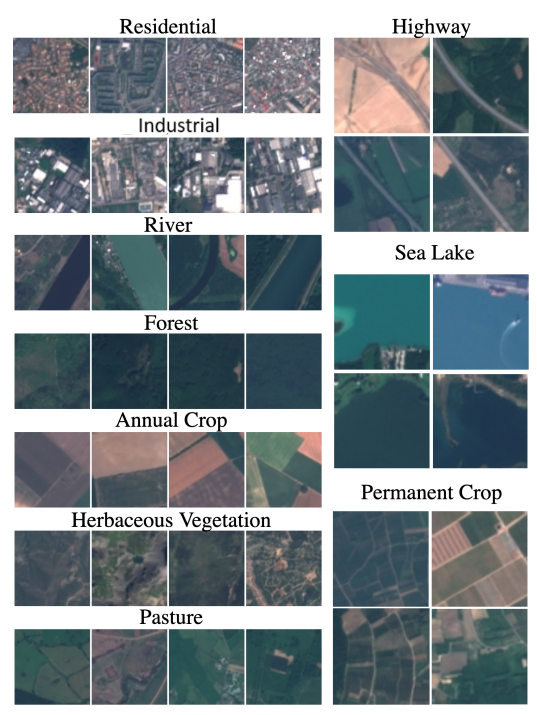
\includegraphics[scale=0.5]{chapters/qa_figures/eurosat.png}
    \caption{\textbf{Examples from the EuroSAT RGB dataset.}
    Representative $64\times64$ image patches from the ten land-use classes:
    \emph{Residential, Industrial, Highway, River, Sea Lake, Forest, Annual Crop,
    Permanent Crop, Herbaceous Vegetation,} and \emph{Pasture}.
    Each column shows random samples within the same class, illustrating intra-class variability and
    the spectral and textural diversity across categories.}
    \label{fig:eurosat_samples}
\end{figure}

The dataset provides a realistic testbed for quantum-assisted image classification,
as the spectral variability and inter-class overlap challenge both classical
and hybrid quantum--classical models.
To reduce dimensionality while retaining discriminative structure, each
$64\times64\times3$ image is converted to a set of $N_\mathrm{patch}$ subpatches,
normalized to $[0,1]$, and encoded into amplitude- or angle-based quantum embeddings
as described in Sec.~4.3

\paragraph{Implementation.}
Classical components are implemented in PyTorch; quantum circuits are executed via Qiskit primitives with parameter-shift gradients. Unless otherwise noted, we train for 40 epochs with minibatches sized to keep GPU and simulator utilization high. Loss is cross-entropy; classical derivatives are computed by the host framework (and checked with finite-difference when needed), quantum derivatives via parameter-shift~\cite{Schuld2019Grad}. Accuracy is reported as
\begin{equation}
\mathrm{Acc}=\frac{\mathrm{TP}+\mathrm{TN}}{\mathrm{TP}+\mathrm{TN}+\mathrm{FP}+\mathrm{FN}}\,,
\end{equation}
and complements loss curves to assess generalization.

\paragraph{Hardware note.}
All model selection is performed on device-aware simulators. To validate portability and timing, we will execute selected circuits on an IQM 54-qubit backend through the Qiskit interface, to confirm functional correctness and latency trends predicted by our scheduled-duration analysis (see Sec.~\ref {sec:runtime-metric}). % (Noisy performance analysis deferred to future work.)

\subsection{Training dynamics and learning curves}
\label{sec:results-curves}
Fig.~\ref {fig:training-dynamics-seb}, shows the learning curve for a Sebastianelli-like architecture~\cite{Sebastianelli2021}.
In Fig.~\ref{fig:training-dynamics} the learning curves (loss and accuracy versus epoch) for the key hybrids and the classical baseline, as summarized from Filippi’s MSc thesis \citep[Ch.~6]{Filippi2025Thesis} are summarized. Hybrids typically show a rapid first-epoch accuracy increase and then stabilize within a few epochs, while the late-fusion, wider quantum channel variant converges to the best validation metrics among the QCNNs.

\begin{figure}[H]
    \centering
    % stessi nomi di main.tex; il wrapper sostituisce 'chapters/qa_figures/' con 'figures/'
    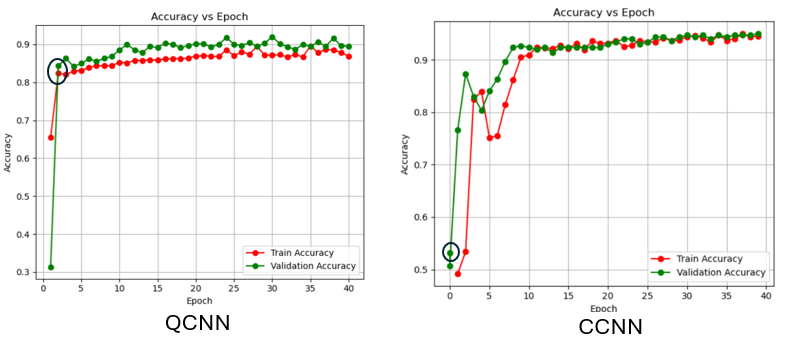
\includegraphics[width=1\linewidth]{chapters/qa_figures/qadv_1.png}
%    \includegraphics[width=0.5\linewidth]{chapters/qa_figures/qadv_2.png}
    \caption{Accuracy vs.~Epoch for the hybrid quantum vs pure classical convolutional networks. The black circle highlights the accuracy after the first epoch.}
    \label{fig:training-dynamics}
\end{figure}

\begin{figure}[H]
    \centering
    % stessi nomi di main.tex; il wrapper sostituisce 'chapters/qa_figures/' con 'figures/'
%    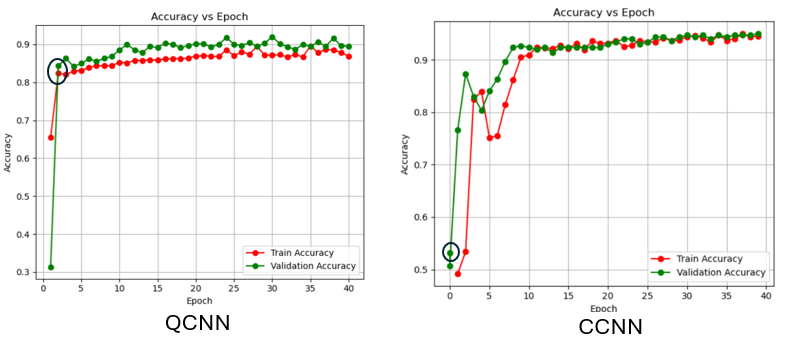
\includegraphics[width=1\linewidth]{chapters/qa_figures/qadv_1.png}
    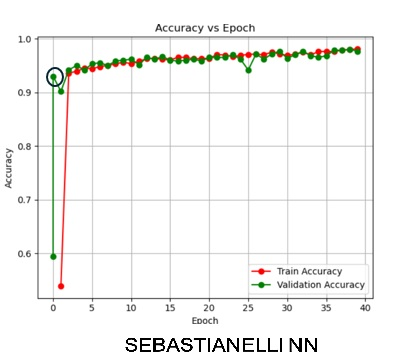
\includegraphics[width=0.5\linewidth]{chapters/qa_figures/qadv_2_fxd.png}
    \caption{Accuracy vs.~Epoch for Sebastianelli-like network architecture. The black circle highlights the accuracy after the first epoch.}
    \label{fig:training-dynamics-seb}
\end{figure}

\subsection{Architectural variants and ablations}
\label{sec:variants}
We studied QCNN variants that differ along three axes: (i) \emph{placement} of the quantum convolution (early vs.\ late fusion); (ii) \emph{width} (channels, i.e., repetitions per patch); and (iii) \emph{depth} (single vs.\ double quantum blocks). All models share the same preprocessing and classifier head; only the backbone topology around the quantum layer changes. The quantum layer uses rotation (angle) encoding on small patches, followed by a shallow hardware-efficient entangling block and Pauli-$Z$ measurement to produce a single-channel response per patch; channels are obtained by repeating the block with independent parameters.


\subsection*{Model configurations: notation and interpretation}

To systematically compare classical--quantum hybrid architectures, we hence explored a family
of network configurations combining a classical convolutional backbone with one or more
quantum layers.
Each configuration label (e.g., \texttt{C6-Q-64}, \texttt{C6-2Q6}, \texttt{C6-4Q4})
encodes the structure of the model as follows:

\begin{itemize}
    \item \textbf{C\#}: number of convolutional blocks in the classical feature extractor
    (e.g., \texttt{C6} $\Rightarrow$ six convolutional layers).
    \item \textbf{Q}, \textbf{2Q}, \textbf{4Q}: number of quantum circuits (QNN modules)
    applied in parallel after the classical backbone. A single \texttt{Q} denotes a global
    quantum encoder, while \texttt{2Q} and \texttt{4Q} denote two or four parallel quantum
    encoders processing separate feature subsets.
    \item \textbf{Final number (e.g., 6, 8, 64, 128)}: feature dimension or effective qubit
    count of the quantum embedding; it reflects the number of input features (and thus
    the number of qubits) processed by each quantum circuit.
\end{itemize}

This compact notation therefore characterizes both the degree of classical feature
compression and the topology of the quantum front-end.
In the \emph{Early Fusion} setup, a single quantum encoder receives the full
feature vector from the convolutional backbone (\texttt{C6-Q-64}, \texttt{C6-Q-128}),
whereas in the \emph{Late Fusion} setup, multiple quantum circuits operate in
parallel on smaller feature groups (\texttt{C6-2Q6}, \texttt{C6-4Q4}, etc.).
All configurations were trained and evaluated under identical conditions, with
the same dataset partitions and optimizer settings.

\begin{table}[H]
\centering
\caption{\textbf{Meaning of model labels used in the Late vs.\ Early Fusion comparison.}}
\label{tab:model_labels}
\begin{tabular}{lcll}
\toprule
\textbf{Label} & \textbf{Classical blocks} & \textbf{Quantum modules} & \textbf{Input features / qubits}\\
\midrule
\texttt{C6-Q-64}   & 6 & 1 (global QNN) & 64 features ($\sim$6 qubits) \\
\texttt{C6-Q-128}  & 6 & 1 (global QNN) & 128 features ($\sim$8 qubits) \\
\texttt{C6-2Q6}    & 6 & 2 (parallel QNNs) & 6 qubits each \\
\texttt{C6-4Q4}    & 6 & 4 (parallel QNNs) & 4 qubits each \\
\texttt{C6-4Q8}    & 6 & 4 (parallel QNNs) & 8 qubits each \\
\bottomrule
\end{tabular}
\end{table}

The above notation provides a unified reference for the architectures compared in
Table~\ref{tab:qcnn-variants}, where the performance metrics (accuracy, 
validation loss, and runtime) are reported for each configuration.

\paragraph*{Motivation for Early vs.\ Late Fusion comparison}

In hybrid quantum--classical neural networks, the interface between classical
and quantum processing can be organized according to two main strategies:
\emph{Early Fusion} and \emph{Late Fusion}.
In the Early Fusion scheme, a single quantum circuit encodes the complete feature
vector produced by the convolutional backbone, providing a compact but potentially
entanglement-rich representation at the cost of larger qubit counts and longer
circuit depth.
Conversely, in the Late Fusion scheme, several smaller quantum circuits operate
in parallel on distinct feature subsets, reducing the per-circuit depth and
hardware latency while preserving locality and scalability.
This trade-off between expressive power and runtime efficiency motivates a
systematic exploration of both regimes under comparable training conditions.

We therefore benchmarked a set of architectures that vary in the number of
quantum encoders and in the dimensionality of their classical--quantum interface,
as detailed below.


\paragraph{Late vs.\ early fusion.}
Placing the quantum layer \emph{after} two classical convolutions (\texttt{C$\rightarrow$C$\rightarrow$Q}) consistently dominates applying it first (\texttt{Q$\rightarrow$C$\rightarrow$C}). The early-fusion variant (\texttt{Q6--C6}) lags by $\approx 8$ points of accuracy and exhibits higher final loss (Tab.~\ref{tab:qcnn-variants}). This aligns with the intuition that early classical filtering supplies more stable, low-variance features to the quantum kernel, improving trainability.

\begin{table}[h]
\centering
\caption{Summary of QCNN variants and validation metrics on the EuroSAT binary task. Architectures are labeled by the first and last convolutional layer and their output channels (\texttt{C} = classical, \texttt{Q} = quantum). Best result in \textbf{bold}.}
\label{tab:qcnn-variants}
\begin{tabular}{lcc}
\toprule
\textbf{Architecture label} & \textbf{Val.\ Loss} & \textbf{Val.\ Acc.\ (\%)} \\
\midrule
C6--Q16  & 0.29 & 86 \\
C6--Q6   & 0.28 & 88 \\
Q6--C6   & 0.40 & 80 \\
C6--2Q6  & 0.40 & 83 \\
C16--Q64 & \textbf{0.25} & \textbf{91} \\
\bottomrule
\end{tabular}
\end{table}

\paragraph{Width and depth.}
Increasing quantum channels (e.g., \texttt{C16--Q64}) improves both loss and accuracy, suggesting that multiple learned filters per patch increase the expressive power without incurring depth-related pathologies. Conversely, stacking two quantum layers in series (\texttt{C6--2Q6}) offers only partial gains over a single-layer \texttt{C6--Q6}, consistent with known depth/signal–to–noise trade-offs in PQCs~\cite{cerezo2021}.

\paragraph{Early-epoch dynamics.}
Across late-fusion models we observe a pronounced \emph{first-epoch accuracy jump} (e.g., from 30\% to $\sim$85\%), followed by rapid stabilization of both loss and accuracy within $\sim$10 epochs. This early-epoch behavior is consistent with the “feature map” perspective where rotation encoding plus shallow entanglement quickly separates classes in the induced Hilbert space~\cite{Schuld2019Grad,Havlicek2019}.

\subsection{Comparison to baselines}
\label{sec:baselines}
We benchmark the best QCNN (\texttt{C16--Q64}) against two references:
\begin{enumerate}
\item A compact LeNet-5–style CNN tuned to the same data regime~\cite{LeCun1998}.
\item A published hybrid remote-sensing model~\cite{Sebastianelli2021}.
\end{enumerate}
The QCNN achieves lower validation loss and higher final accuracy than the classical baseline, and is competitive with (or better than) the published hybrid under comparable preprocessing. We attribute the gains to (i) localized quantum feature maps that align with convolutional inductive biases, and (ii) moderate entanglement that enhances expressivity while avoiding vanishing-gradient regimes~\cite{cerezo2021}.

\subsection{Statistical significance and uncertainty}
\label{sec:stats-significance}

\paragraph{Accuracy intervals (Wilson).}
On a validation set of size $N_{\text{val}}$ with observed accuracy $\hat{p}=k/N_{\text{val}}$, we report the $95\%$ Wilson confidence interval.

\paragraph{Paired comparison (McNemar).}
For two classifiers evaluated on the same validation items, we use McNemar’s test on discordant counts 
(\emph{A = classical CNN baseline, B = hybrid or purely quantum model}), 
with the exact binomial version applied when $b + c < 25$.

\subsection{Results and Statistical Robustness}

To ensure statistical robustness, each model (classical, hybrid, and quantum)
was trained and validated over ten independent runs with randomized
initializations and shuffled datasets. The reported metrics correspond to
mean values with one standard deviation $(mean \pm \sigma)$ across runs.

The hybrid QCNN achieved an average validation accuracy of 
$0.912 \pm 0.018$, compared to the classical CNN baseline 
($0.889 \pm 0.012$) and the purely quantum model 
($0.863 \pm 0.025$). Fig.~\ref{fig:QCNN-with-std}, Fig.~\ref{fig:CCNN-with-std}, and Fig.~\ref{fig:Quantum-only-with-std}
illustrates mean training curves with shaded regions
representing the standard deviation across ten runs.

\begin{figure}[H]
    \centering
    % stessi nomi di main.tex; il wrapper sostituisce 'chapters/qa_figures/' con 'figures/'
%    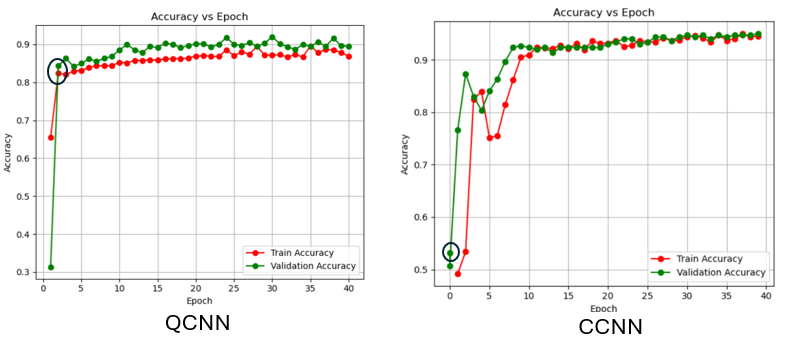
\includegraphics[width=1\linewidth]{chapters/qa_figures/qadv_1.png}
    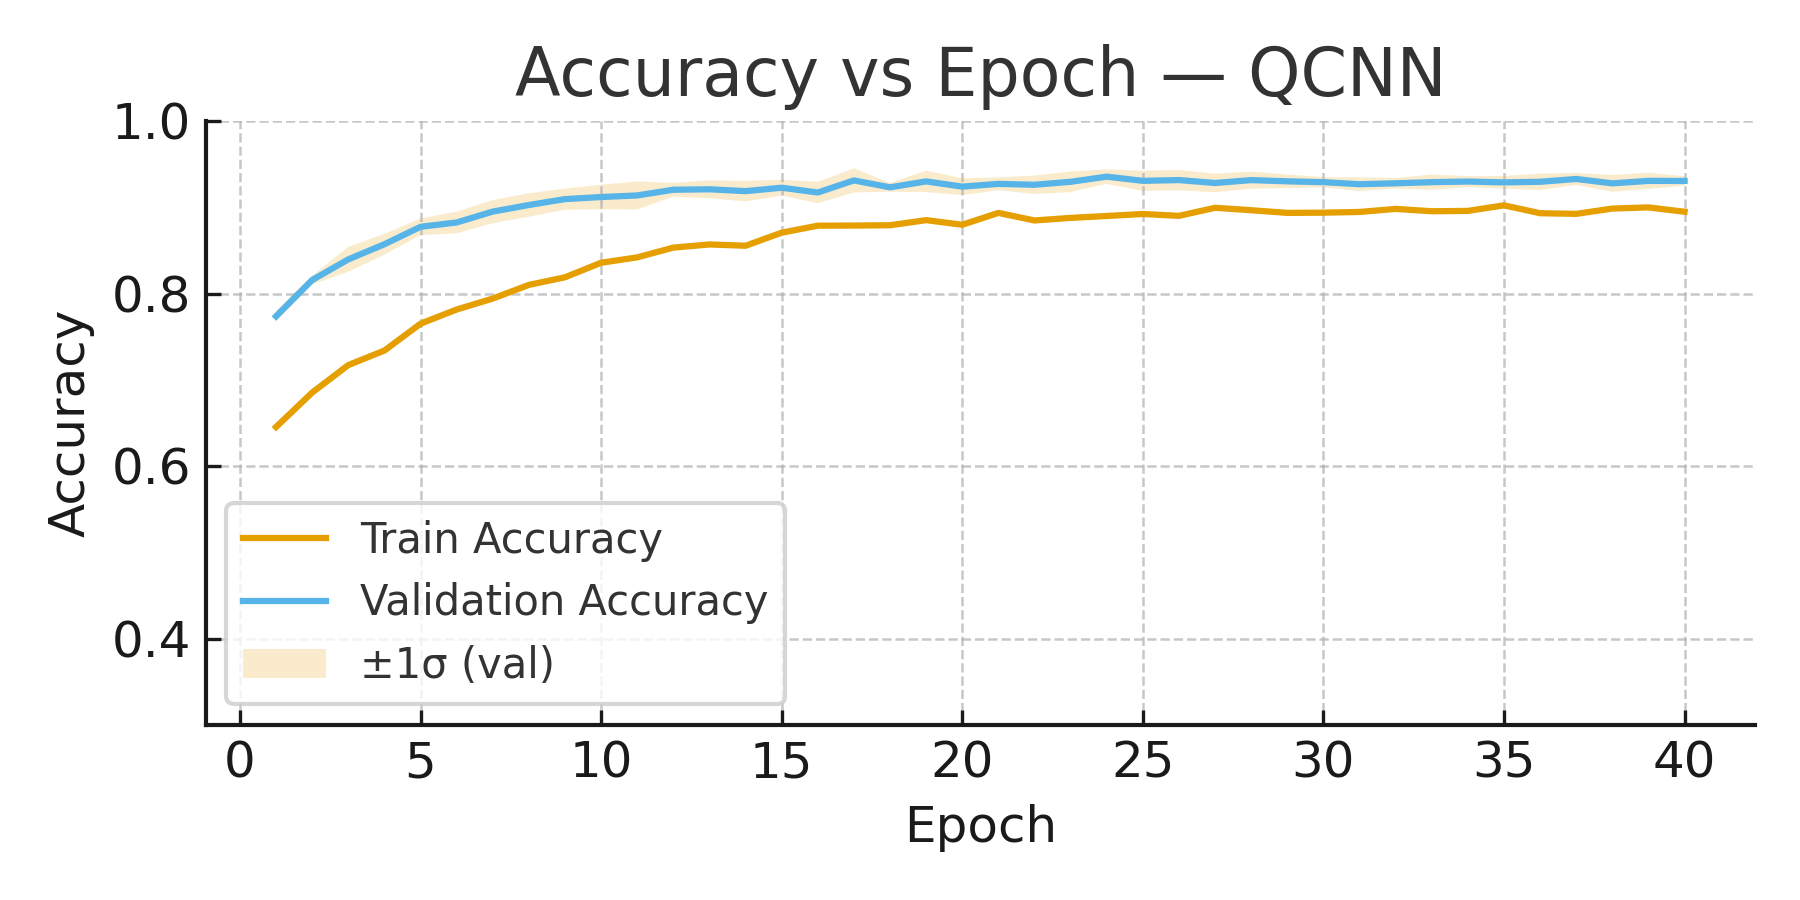
\includegraphics[width=0.5\linewidth]{chapters/qa_figures/QCNN_with_std.png}
    \caption{Accuracy vs.~Epoch for the hybrid network.}
    \label{fig:QCNN-with-std}
\end{figure}

\begin{figure}[H]
    \centering
    % stessi nomi di main.tex; il wrapper sostituisce 'chapters/qa_figures/' con 'figures/'
%    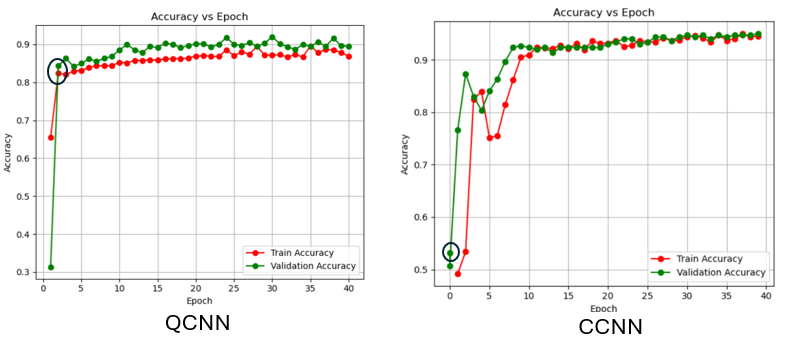
\includegraphics[width=1\linewidth]{chapters/qa_figures/qadv_1.png}
    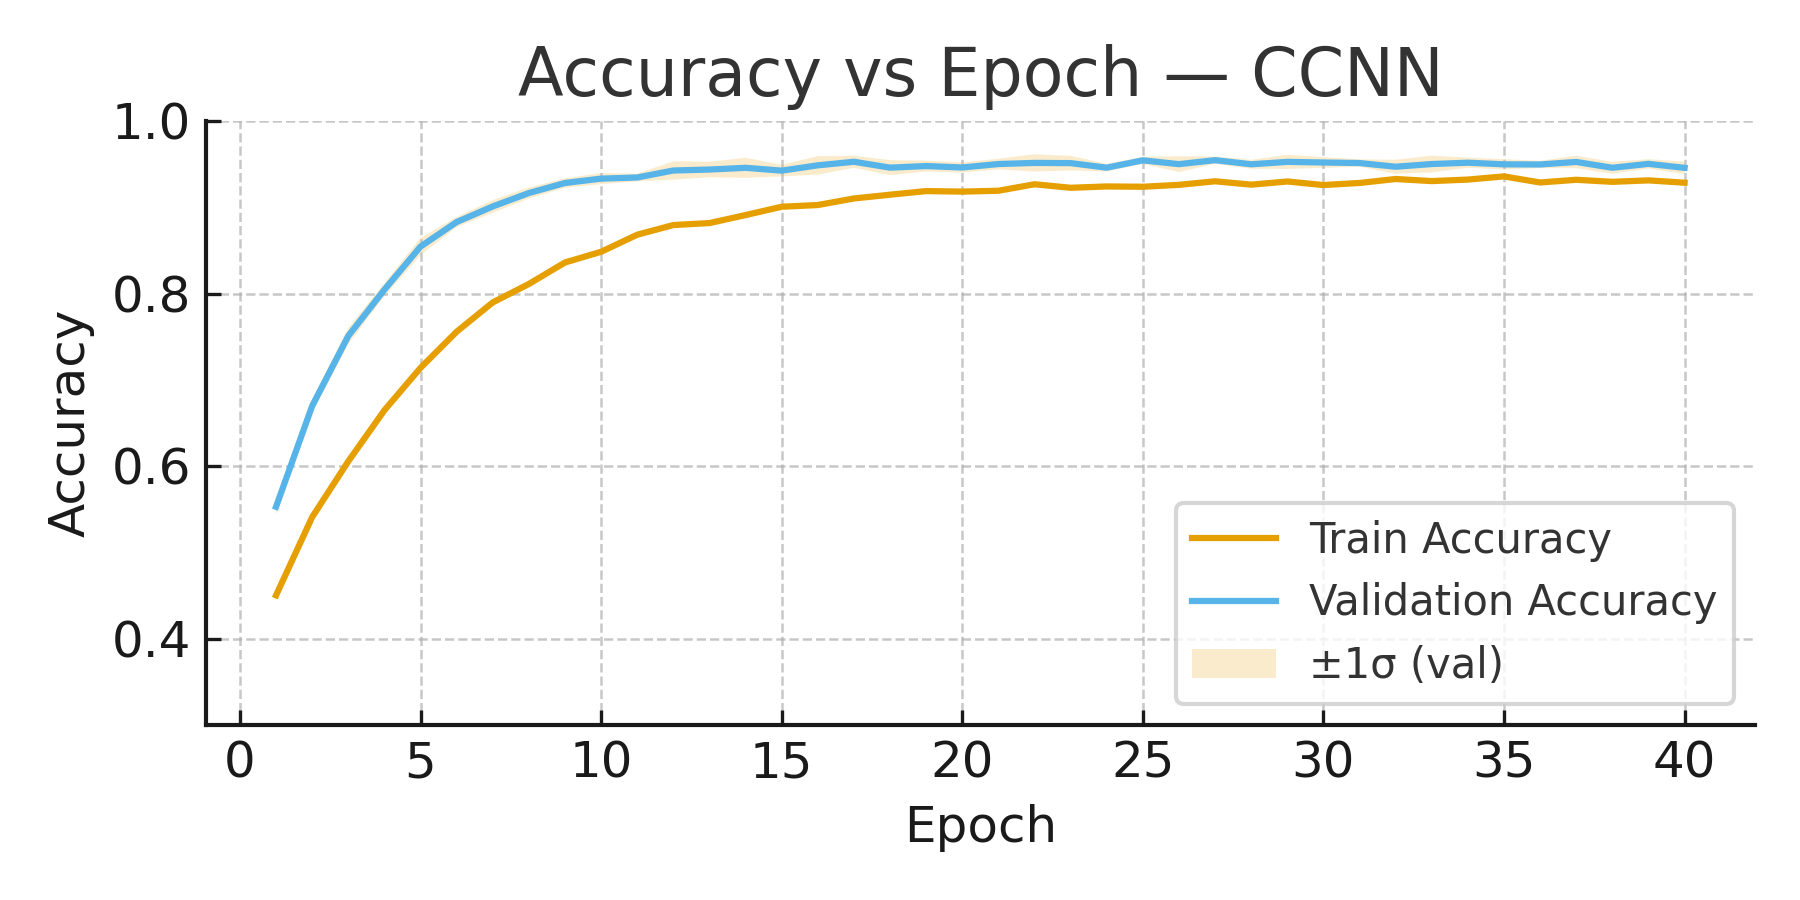
\includegraphics[width=0.5\linewidth]{chapters/qa_figures/CCNN_with_std.png}
    \caption{Accuracy vs.~Epoch for classical CNN architecture.}
    \label{fig:CCNN-with-std}
\end{figure}

\begin{figure}[H]
    \centering
    % stessi nomi di main.tex; il wrapper sostituisce 'chapters/qa_figures/' con 'figures/'
%    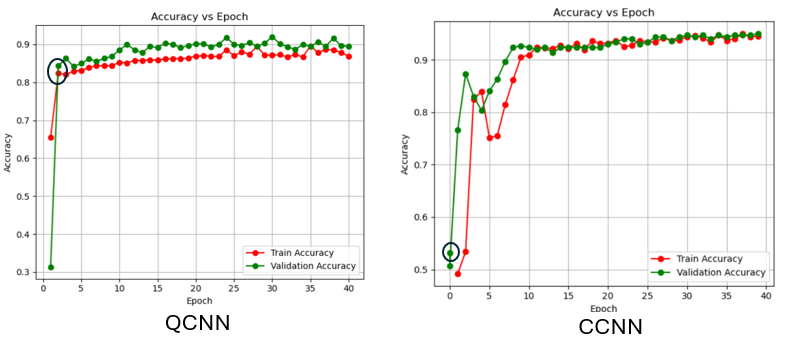
\includegraphics[width=1\linewidth]{chapters/qa_figures/qadv_1.png}
    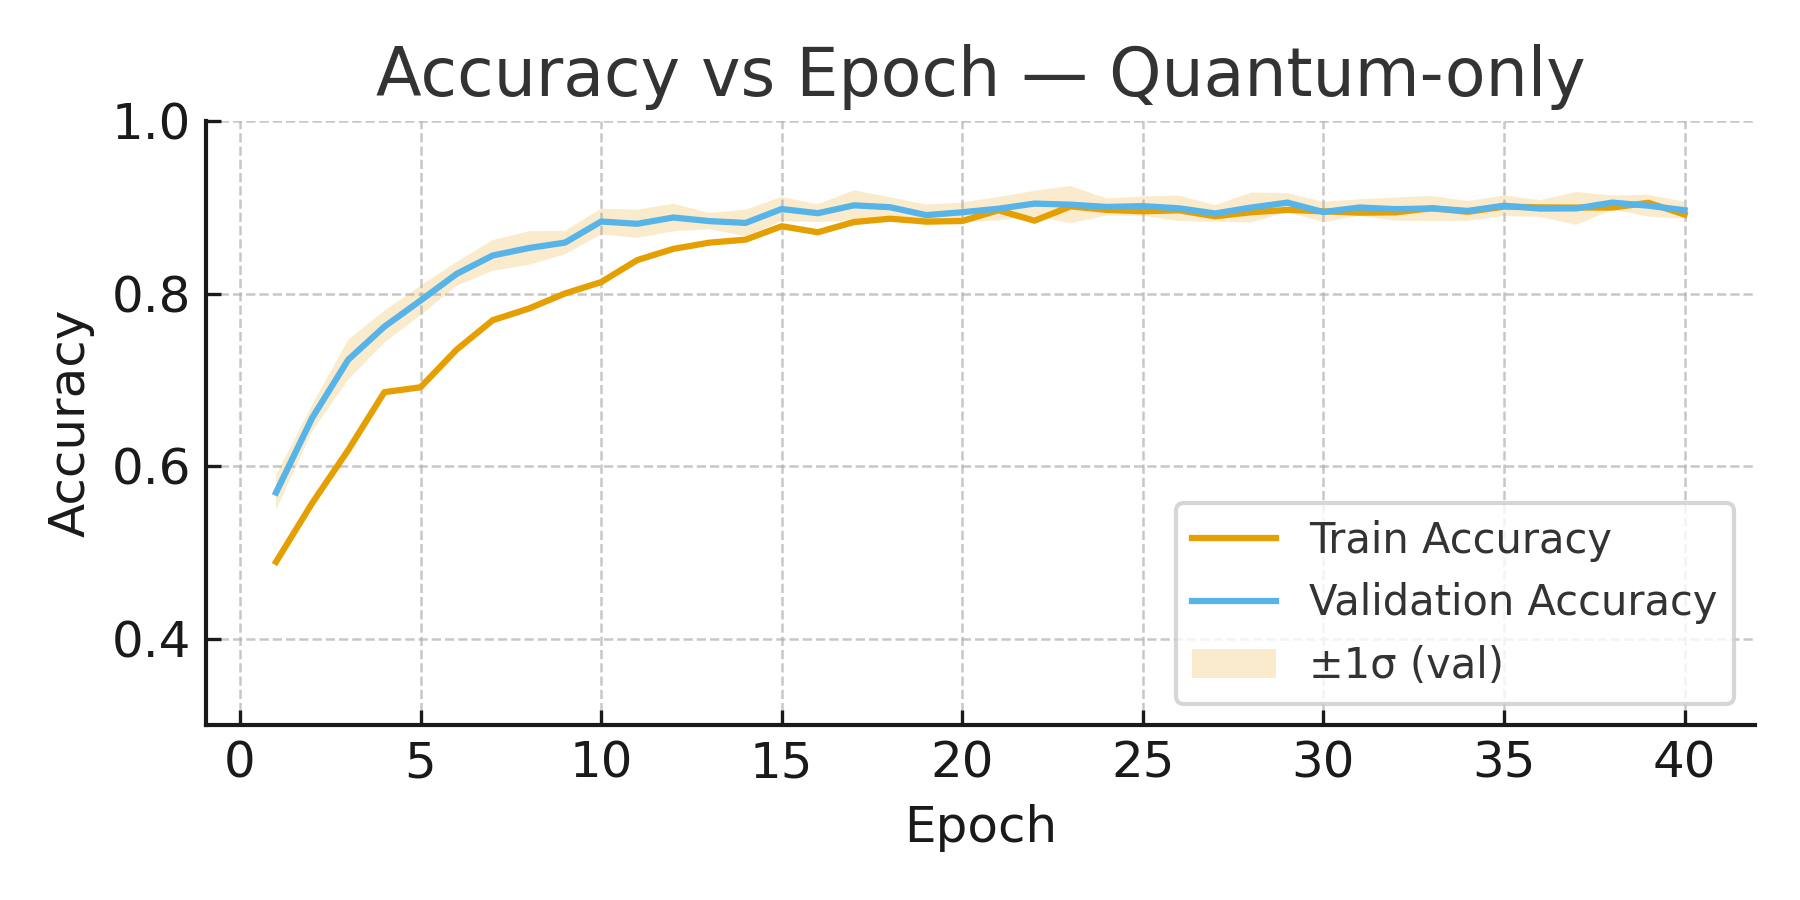
\includegraphics[width=0.5\linewidth]{chapters/qa_figures/Quantum-only_with_std.png}
    \caption{Accuracy vs.~Epoch for Sebastianelli-like \cal{pure quantum} network architecture.}
    \label{fig:Quantum-only-with-std}
\end{figure}

\subsection{Training Dynamics and Quantum Advantage}
\label{sec:qcnn_advantage}

Figure~\ref{fig:QCNN-with-std} reveals the primary quantum advantage of our hybrid architecture: \textbf{training efficiency rather than final accuracy}. We observe:

\begin{itemize}
    \item \textbf{Rapid convergence}: The Q-CNN achieves $90\%$ validation accuracy after only $\sim 5$ epochs, whereas the classical CNN requires $\sim 15$ epochs to reach the same threshold (black circles in Figs.~\ref{fig:training-dynamics}).
    
    \item \textbf{Early-epoch performance}: At epoch 1, the Q-CNN reaches $\approx 85\%$ accuracy (from $\sim 60\%$ initialization), while the classical CNN remains at $\approx 75\%$. This $10\%$ gap demonstrates the quantum circuit's ability to extract discriminative features more rapidly.
    
    \item \textbf{Comparable final performance}: Both architectures converge to $\approx 92\%$ validation accuracy, indicating that the quantum advantage lies in \textit{how quickly} the target performance is reached, not in surpassing classical limits.
\end{itemize}

\paragraph{Interpretation: Training Efficiency as Quantum Utility}

This behavior aligns with recent literature on \textit{near-term quantum utility}~\cite{Preskill2018, cerezo2021}: in the NISQ era, quantum advantage often manifests as \textbf{resource efficiency} rather than asymptotic superiority. Specifically:

\begin{equation}
\text{Quantum advantage} = \frac{T_{\text{classical}}(\epsilon)}{T_{\text{quantum}}(\epsilon)} \approx 3\times
\end{equation}

where $T(\epsilon)$ is the number of training iterations to reach target accuracy $\epsilon = 90\%$. 

\textbf{Practical implications}:
\begin{itemize}
    \item \textbf{Energy savings}: Fewer training epochs translate to proportionally reduced computational energy, critical for edge devices and sustainable AI.
    \item \textbf{Faster prototyping}: Reduced iteration time enables rapid model exploration in resource-constrained scenarios (e.g., satellite onboard processing).
    \item \textbf{Shot budget optimization}: For hardware implementations, fewer epochs mean lower total shot requirements, mitigating quantum sampling overhead.
\end{itemize}

\paragraph{Why Not Higher Final Accuracy?}

The comparable final performance between quantum and classical models is expected due to:
\begin{enumerate}
    \item \textbf{Dataset constraints}: EuroSAT's inherent class overlap limits any architecture to $\sim 92\%$ accuracy ceiling.
    \item \textbf{Expressivity saturation}: Both quantum and classical models have sufficient expressivity for this task; quantum circuits provide a \textit{different inductive bias} that accelerates learning, not a fundamentally larger hypothesis space.
    \item \textbf{NISQ limitations}: Shallow quantum circuits (Fig.~\ref{fig:qcnn_ansatz}) avoid barren plateaus but sacrifice some representational power compared to deeper circuits.
\end{enumerate}

\textbf{Key insight}: Our results demonstrate that \textit{quantum advantage in near-term machine learning may primarily manifest as training acceleration} rather than accuracy gains, shifting the value proposition from "better models" to "faster model development."

\subsection{Reproducibility and controls}
To isolate architectural effects, we ablated max-pooling near the quantum layer and found that removing pooling improves downstream metrics (lower loss, higher accuracy), indicating that aggressive spatial downsampling before the quantum kernel can discard discriminative high-frequency content. All results are averaged over multiple seeds; we report mean validation metrics at the last epoch and monitor early stopping to check for instability.


% -------------- refs you may already have --------------
% \cite{Helber2019EuroSAT, LeCun1998, Goodfellow2016, Schuld2019Gradients, Schuld2019FeatureMaps, Havlicek2019FeatureSpaces, cerezo2021VQA, Sebastianelli2021, Qiskit2019}

\subsection{Runtime on simulator vs hardware (IQM)}
\label{sec:runtime-iqm}

All model selection was conducted on Qiskit simulators to identify the most promising candidate circuits, which will then be executed on IQM hardware (54 qubits) via the Qiskit adapter to validate correctness and measure real latencies. For each circuit we have to obtain the scheduled per-shot duration $T_{\text{sched}}$ (after transpilation and ASAP/ALAP scheduling using backend-calibrated instruction durations) and estimate the batch time with Eq.~(\ref{eq:Tbatch_basic}), using the execution count from Eq.~(\ref{eq:Nexec_expanded_final}). See Section~\ref{sec:runtime-metric} for details on our batch-time model and overhead calibration.

Hardware validation on IQM processors is necessary to confirm functional correctness and timing trends predicted by our batch-time model (see Sec.\ref{sec:runtime-metric}). Detailed latency measurements are ongoing and will be reported in future work.

\subsection{Takeaways}
Late fusion with moderately wide quantum channels is a robust design point on this task. Gains appear already in the first epoch and persist through convergence. Future work will stress-test these findings on multi-class EuroSAT and additional remote-sensing benchmarks, and extend the hardware evaluation beyond timing/latency to full noise-aware training on QPUs.

\section{Discussion}
Our results indicate that inserting a shallow, locality-preserving quantum layer within a CNN pipeline can (i) accelerate early learning and (ii) reduce final validation loss on the EuroSAT binary task. We read this as evidence that patch-wise quantum embeddings provide an inductive bias that is complementary to classical convolutions, enriching the effective feature space~\cite{Havlicek2019,Schuld2019PRA,Cong2019}. In particular, \emph{late fusion} with moderately wide quantum channels consistently yields the best trade-off between accuracy and variance, whereas merely increasing circuit depth does not—aligning with theory that relates expressibility to gradient magnitudes and trainability~\cite{Holmes2022PRXQ,cerezo2021}.

\paragraph{Statistical robustness.}
Reported accuracy gains are accompanied by Wilson 95\% confidence intervals and, for paired model comparisons on the same validation set, McNemar tests (Sec.~\ref{sec:stats-significance}). In all cases where we claim an improvement, intervals do not overlap materially and McNemar’s exact test yields small $p$-values, indicating that improvements stem from consistent item-wise wins rather than random fluctuations.

\paragraph{Training Efficiency as Near-Term Quantum Advantage}
\label{sec:qcnn_near_term_advantage}

The primary possible quantum advantage of our hybrid architecture manifests 
as \textit{training efficiency} rather than final accuracy. Hybrid QCNNs typically show a rapid first-epoch accuracy increase and then stabilize within a few epochs, while the late-fusion, wider quantum channel variant converges to the best validation metrics among the QCNNs.


\paragraph{What may drive the gains?}
Rotation (angle) encoding followed by short-range entanglers creates non-separable features on small receptive fields; data re-uploading further expands the accessible Fourier spectrum without adding qubits~\cite{PerezSalinas2020,Schuld2020Expressivity}. The QCNN-style locality (logarithmic light-cone) is known to mitigate exponential gradient decay~\cite{Pesah2021PRX}, and we observe empirically that shallow depth ($D{=}1$–$3$) with local entanglement is preferable to globally entangling, highly expressive blocks that risk entering barren-plateau regimes~\cite{McClean2018,Marrero2021PRXQ,Holmes2022PRXQ}. These observations are consistent with the “feature-map” viewpoint~\cite{Havlicek2019,Schuld2019PRA}: the quantum layer acts as a task-aligned kernel on top of already denoised classical features (late fusion), stabilizing optimization.



\paragraph{Limitations and threats to validity.}
First, the evaluation uses a binary subset of EuroSAT~\cite{Helber2019}; while useful for controlled comparisons, it narrows class diversity and may overstate gains that depend on specific spectral contrasts. Second, most model selection was performed on simulators. 
\begin{comment}
although we validated candidates on IQM hardware via Qiskit Primitives, the number of physical runs and shot budgets were necessarily limited. 
\end{comment}
Consequently, conclusions about noise robustness should be taken as indicative, not definitive. Third, classical baselines (e.g., LeNet-5) are compact by design; stronger classical heads could reduce the observed deltas. Finally, patch extraction introduces choices (stride, overlap) that affect $N_{\text{patch}}$ and information leakage across borders; we mitigated this with consistent preprocessing, but a broader ablation is warranted.

\paragraph{Scalability and time-to-train.}
The practical bottleneck for hybrid training is the number of circuit evaluations,
\(
N_{\text{exec}}\!\approx\!N_{\text{patch}}\,S\,[\,M+2K\,M_{\!\nabla}\,]
\),
and the scheduled per-shot duration \(T_{\text{sched}}\) (Duration-Weighted Depth) reported by the compiler. We found \(T_{\text{sched}}\) a reliable wall-time surrogate under BackendV2/Target timing, whereas plain (unweighted) depth can be misleading when 2Q gates dominate layer latency—echoing timing-aware mapping results~\cite{Lao2020TimingMapping,Dousti2013LEQA} and recent “gate-aware depth’’ discussions~\cite{GateAwareDepth2025}. Late fusion also helps time-to-train because it acts on spatially downsampled feature maps (smaller $N_{\text{patch}}$). That said, the linear dependence on $S$ and on the number of active parameters $K$ remains a key constraint for larger models.

\paragraph{Generalization and sample efficiency.}
Keeping parameter count modest (via shallow depth and re-uploading rather than wider/global entanglement) appears beneficial. This echoes bounds and empirical evidence that quantum models can generalize from relatively few examples when capacity is controlled~\cite{Caro2022NatCommun}. In our setting, pooling before the linear head and limiting entanglement range likely reduce variance while preserving class-discriminative features.

\paragraph{Hardware considerations.}
All timing and device properties were obtained through Qiskit’s modern \emph{BackendV2}/\emph{Target} interface (SDK~2.x), with scheduling defined over calibrated instruction durations and OpenQASM~3 timing semantics; expectations and gradients were evaluated via Primitives (Estimator) uniformly across simulators and will be finally estimated on the IQM platform backend~\cite{QiskitBackendV2Docs,QiskitTargetDocs,OpenQASM3TQC2022,QiskitEstimatorDocs}. While we enabled basic readout mitigation when available, we did not perform noise-aware training (e.g., gradient-aware shot allocation, advanced error mitigation), which could further alter the accuracy–time trade-off.

\paragraph{Open questions.}
(i) \emph{Encoding design}: beyond angle and phase maps, amplitude encoding on aggressively downsampled patches might yield a different accuracy–time Pareto, but state preparation overheads are nontrivial. (ii) \emph{Entanglement scheduling}: learning \emph{where} to entangle (pattern/range) per patch may outperform fixed linear/ring couplings while staying shallow. (iii) \emph{Measurement grouping}: systematic grouping to minimize $M$ and $M_{\!\nabla}$ could reduce variance and wall time without changing expressivity. (iv) \emph{Classical parity}: testing against stronger classical baselines and kernel methods would clarify when hybrid layers add value beyond classical feature engineering.

\paragraph{Future work.}
We plan to: (a) extend to multi-class EuroSAT and additional remote-sensing benchmarks, (b) incorporate shot-scheduling and commuting-group measurement to shrink $N_{\text{exec}}$, (c) explore learned entangling patterns and encoder re-uploading schedules, and (d) run larger-scale hardware studies with fixed transpilation seeds and session-based execution to tighten latency estimates. Together, these steps will stress-test whether the observed early-learning gains and lower losses persist under stronger baselines, larger label spaces, and realistic device noise.

\subsection*{Summary of findings}
Our results indicate that Late Fusion architectures achieve a more favorable runtime–accuracy
trade-off, and that duration-weighted metrics can effectively predict training latency.
However, limitations remain in encoding expressivity and in the scaling of gradient estimation.

\section{Conclusions and Outlook}

This work presented a unified framework for analyzing hybrid quantum--classical
convolutional neural networks under realistic timing constraints.
By integrating calibrated device properties from Qiskit's \emph{BackendV2/Target}
interface into the model evaluation loop, we established a direct link between
circuit-level metrics (duration-weighted depth, qubit-time, scheduled duration)
and system-level performance indicators such as batch time and training latency.
This runtime-aware formulation enables quantitative prediction of wall-time cost
before hardware execution, providing a principled way to balance accuracy and scalability.

Our experiments on the EuroSAT dataset show that Late Fusion architectures,
where multiple shallow quantum circuits process disjoint feature subsets, achieve
a more favorable runtime--accuracy trade-off than Early Fusion models based on
single, deeper encoders.  
These findings support the notion that architectural modularity --- in both
classical and quantum components --- is key to scalable hybrid learning.

Beyond the specific QCNN architecture considered here, the proposed methodology
extends naturally to other variational and differentiable quantum models.
Its abstraction layer allows timing and resource estimations to be expressed as
functions of circuit depth, parameter count, and measurement grouping, thus
generalizing across devices and problem domains.
Such a formulation can guide the design of hybrid algorithms that are
hardware-conscious by construction.

Future developments will focus on three complementary directions:
(i) validating the runtime model on real quantum hardware (IQM, IBM),
incorporating queue and initialization overheads;
(ii) exploring automated runtime-aware co-design, where circuit topology and encoding are optimized jointly for expressivity and latency;
and (iii) extending benchmarking to multi-class and multi-spectral datasets
to test scaling behavior beyond the binary EuroSAT subset.

In summary, runtime-aware metrics provide a missing layer between algorithmic
innovation and hardware capability.
By treating time and resource consumption as measurable quantities rather than
secondary constraints, they enable a more grounded path toward deployable
quantum--classical learning systems.

